\documentclass[type=bsc,accentcolor=tud9c]{tudthesis}
\usepackage[utf8]{inputenc}
\usepackage[hyphens]{url}
\usepackage{hyperref}
\usepackage[nottoc,numbib]{tocbibind}
\usepackage{mdframed}
\usepackage{array}
\usepackage{minted}
\usepackage{tikz}
\usepackage{pdfpages}
\usepackage{listings}
\usepackage[font=small,labelfont=bf]{caption}
\usepackage{chngcntr}
\usepackage{enumitem}
\usepackage{longtable}
\usepackage{subcaption}
\usepackage{rotating}
\usepackage[doublespacing]{setspace}
\usepackage[normalem]{ulem}
\usetikzlibrary{arrows,shapes,positioning,shadows,trees} % x-y Diagrams

\newcommand{\framework}[1]{\textcolor{black!65}{#1}}
\usemintedstyle{trac}
%Change Bibliografy name to References
\renewcommand\bibname{References}

\newcommand{\inputjava}[2]{\inputminted[frame=lines,framesep=2mm,linenos,frame=single,fontsize=\small, breaklines=true,highlightcolor=\myMarkerColor, highlightlines={#1}]{java}{#2}}
\newcommand{\inputcode}[2]{\inputminted[frame=lines,framesep=2mm,linenos,frame=single,fontsize=\small, breaklines=true,highlightcolor=\myMarkerColor, highlightlines={#1}]{text}{#2}}
\newcommand{\inputftl}[2]{\inputminted[frame=lines,framesep=2mm,linenos,frame=single,fontsize=\small, breaklines=true,highlightcolor=\myMarkerColor, highlightlines={#1}]{text}{#2}}

\newcolumntype{L}[1]{>{\raggedright\let\newline\\\arraybackslash\hspace{0pt}}m{#1}}
\newcolumntype{C}[1]{>{\centering\let\newline\\\arraybackslash\hspace{0pt}}m{#1}}
\newcolumntype{R}[1]{>{\raggedleft\let\newline\\\arraybackslash\hspace{0pt}}m{#1}}

\newcommand{\myMarkerColor}{yellow!30}
\renewcommand{\theFancyVerbLine}{\sffamily\textcolor{black!20}{\scriptsize\oldstylenums{\arabic{FancyVerbLine}}}}

% Command to add notes
\newenvironment{note}
{\begin{mdframed}[backgroundcolor=\myMarkerColor, linewidth=1pt]}
{\end{mdframed}}
\makeatother


% Paper
\newenvironment{sketch}
{\begin{mdframed}[backgroundcolor=gray!30, linewidth=1pt]\itshape}
{\end{mdframed}}
\makeatother

% Java
\newcommand{\removeSpaces}[1]{%
  \begingroup
  \spaceskip=1sp
  \xspaceskip=1sp
  #1%
  \endgroup}

\newcommand{\java}[1]{\removeSpaces{\mintinline{java}{#1}}}
%\newcommand{\code}[1]{\removeSpaces{\mintinline{text}{#1}}}
\newcommand{\code}[1]{\lstinline[basicstyle=\ttfamily\color{black!65}]|#1|}

\newenvironment{javacode}[1]{%
  \VerbatimEnvironment
  \begin{center}%
  	\vspace{0mm}
    \begin{minipage}{\textwidth}%
      \begin{minted}[tabsize=2,frame=lines,framesep=2mm,rulecolor=\color{black!10},linenos,frame=single,fontsize=\footnotesize, breaklines=true,highlightcolor=\myMarkerColor, highlightlines={#1}]{java}}
{%
      \end{minted}%
    \end{minipage}%
  \end{center}}
\makeatother

\newenvironment{textcode}[1]{%
  \VerbatimEnvironment
  \begin{center}%
  	\vspace{0mm}
    \begin{minipage}{\textwidth}%
      \begin{minted}[tabsize=2,frame=lines,framesep=2mm,rulecolor=\color{black!10},linenos,frame=single,fontsize=\footnotesize, breaklines=true,highlightcolor=\myMarkerColor, highlightlines={#1}]{text}}
{%
      \end{minted}%
    \end{minipage}%
  \end{center}}
\makeatother

\newenvironment{javacodemultipage}[1]{%
  \VerbatimEnvironment
  \begin{center}%
	\begin{minted}[frame=lines,framesep=2mm,rulecolor=\color{black!10},linenos,frame=single,fontsize=\footnotesize, breaklines=true,highlightcolor=\myMarkerColor, highlightlines={#1}]{java}}
{%
	\end{minted}%
  \end{center}}
\makeatother

\newenvironment{textcodemultipage}[1]{%
  \VerbatimEnvironment
  \begin{center}%
  	\vspace{0mm}
      \begin{minted}[frame=lines,framesep=2mm,rulecolor=\color{black!10},linenos,frame=single,fontsize=\footnotesize, breaklines=true,highlightcolor=\myMarkerColor, highlightlines={#1}]{text}}
{%
      \end{minted}%
  \end{center}}
\makeatother

\newenvironment{jscode}[1]{%
  \VerbatimEnvironment
  \begin{center}%
  	\vspace{0mm}
    \begin{minipage}{\textwidth}%
      \begin{minted}[tabsize=2,frame=lines,framesep=2mm,rulecolor=\color{black!10},linenos,frame=single,fontsize=\footnotesize, breaklines=true,highlightcolor=\myMarkerColor, highlightlines={#1}]{html}}
{%
      \end{minted}%
    \end{minipage}%
  \end{center}}
\makeatother


\newenvironment{sourcecode}{\captionsetup{type=lstlisting}}{}
\newcommand{\toolcore}{\textsc{2Rx}}
\newcommand{\toolextension}{\textsc{SwingWorker2Rx}}


\begin{document}
%\setstretch{2.5}% for comments
\setstretch{1}% normal
\counterwithin{lstlisting}{chapter}
\counterwithin{figure}{chapter}
\counterwithin{table}{chapter}
\setlist[itemize]{noitemsep}
\setlist[itemize]{nolistsep}
\setlist[enumerate]{noitemsep}
\setlist[enumerate]{nolistsep}

\thesistitle{Automated Refactoring for Asynchronous Applications}{}
\author{Grebiel José Ifill Brito}
\birthplace{Caracas, Venezuela}
\date{February 2017}
\referee{Prof. Dr. Guido Salvaneschi}{xyz}
\department{Computer Science}
\group{Software Technology Group}

\makethesistitle

\chapter*{Summary}
Modern languages are replacing the traditional callback-based approach with method chaining. Some of these languages are using event-driven and reactive programming models~\cite{agera, reactiveX, paperFlapjax}. According to previous studies, these programming paradigms improve code writing and code comprehension~\cite{promises, paperReactiveComprehension}.

Motivated by these facts, we propose an approach that facilitates introducing reactive programming concepts in existing \framework{Java} applications. In order to do that, we transform the source code, so that it uses the \framework{ReactiveX} API. 

We divide the transformation into two steps. First, we modify the source code automatically into an implementation based on the \framework{ReactiveX} API. This transformation does not change the behavior of the program. The second step consists in introducing the reactive programming model into the source code. This part depends on specific requirements. Therefore, one must apply these changes by hand. However, since \framework{ReactiveX} is optimized for the implementation of reactive models~\cite{reactiveX}, adding such concepts in this step is more intuitive for developers. This thesis focuses on the transformation of \code{SwingWorker}s. However, one can extrapolate this approach to other constructs. 

In this work we also present \toolcore{} and \toolextension{}. We developed these tools for the automated modification of the source code. \toolcore{} is the core of the system and \toolextension{} is the extension in charge of converting \code{SwingWorker}s into an implementation that uses \framework{ReactiveX}. 

We evaluate the accuracy of \toolextension{} using 58 projects. The results show that the tool is highly accurate. The limitations of \toolextension{} correspond to particular implementations of \code{SwingWorker}s. Furthermore, we evaluate the flexibility of \toolcore{} to support extensions by adapting \textsc{RxFactor}~\cite{thesisRxFactor} to be its client (extension). \textsc{RxFactor} is a similar tool which goal is to transform \code{AsyncTask}s into an implementation that uses \framework{ReactiveX} as well.

\code{SwingWorker}s and \code{AsyncTask}s are not the only types of constructs available for asynchronous programming. One can implement operations that do not require any synchronization between threads by simply using the \framework{Java} classes \code{Thread} and \code{Runnable}. We suggest the evaluation of these constructs in further research in order identify implementation patterns and design algorithms to transform the code, so it uses \framework{ReactiveX} instead. Moreover, other constructs which are not necessarily related to asynchronous execution could also benefit from the \framework{ReactiveX} API. Since \framework{ReactiveX} supports working with data streams, \code{for-} and \code{while-}loops are also good candidates for this transformation. We encourage future work not only identifying patterns and designing the algorithms but also implementing the corresponding extensions for \toolcore{}, in order to have a single tool which is able to refactor several constructs to \framework{ReactiveX}.

\tableofcontents
\listoffigures
\listoftables
\listoflistings


\chapter{Introduction}
\label{chapter:introduction}
Most UI frameworks are single threaded ~\cite{uiSingleThreaded}. When a long-running operation is executed in the UI thread, then the user interface freezes until the operation has completed. To avoid this blocking behavior, developers use a background thread for these operations.

Several tools have been developed in the last years to automatically modify the source code of asynchronous applications without changing the semantic of the program. This transformation is called refactoring. \textsc{Asynchronizer}~\cite{paperRetrofittingConcurrency}, \textsc{AsyncDroid}~\cite{paperStudyRefactoring}, \textsc{Asyncifier}~\cite{paperAsyncMobile}, \textsc{AsyncFixer}~\cite{paperAsyncMobile}, \textsc{PromisesLand}~\cite{thesisJavaScript} and \textsc{RxFactor}~\cite{thesisRxFactor} are some of these tools. Each of them try to solve different problems. \textsc{Asynchronizer} and \textsc{AsyncDroid} focus on performance improvement in \framework{Android} applications, while \textsc{Asyncfier} and \textsc{PromissesLand} aim increasing the code readability in \framework{C\#} and \framework{JavaScript} respectively. \textsc{AsyncFixer} helps finding and correcting anti patterns of async constructs in \framework{C\#}. Finally \textsc{RxFactor} is a refactoring tool that converts \code{AsyncTask}s into an implementation that uses the \framework{ReactiveX} API. \textsc{RxFactor} was developed parallel to this thesis by another author.

Furthermore, functional programming has been gaining popularity in the last years. \framework{Java 8}, for example, offers several classes to support working with data streams in a functional fashion~\cite{bookJava8Streams}. Other technologies such as \framework{Flapjax}, \framework{ReactiveX} and \framework{Agera} are not only using functional concepts but also focusing on the reactive programming paradigm. \framework{Flapjax} is a programming language that introduces event-driven reactivity as the natural programming model for web applications~\cite{paperFlapjax}. \framework{ReactiveX} is a library based on the observer pattern that supports data streams and functional programming~\cite{reactiveX}. \framework{Agera} also offers classes for functional, asynchronous and reactive programming in \framework{Android} applications~\cite{agera}.

Since reactive and functional programming paradigms facilitate code writing and code comprehension~\cite{promises, paperReactiveComprehension}, it makes sense to refactor existing applications to make the implementation of these programming models easier. We present a refactoring approach to achieve that by using the \framework{ReactiveX} API extension for \framework{Java} called \framework{RxJava}. To decrease the effort required to perform such a refactoring, we developed \toolcore{} and an extension for it \toolextension{}. These tools work together to automatically refactor \code{SwingWorker}s.

The combination of \toolcore{} and \toolextension{} produces a tool which is very similar to \textsc{RxFactor}. The objective of both is to enable functional and reactive programming constructs in existing applications. However, the refactoring approaches and the architectures of these tools are different. In contrast to \textsc{RxFactor}, which is not able to refactor all method invocations available in \code{AsyncTask}s, \toolextension{} supports all methods specified in the \code{SwingWorker} API. The architecture of \toolcore{}, core and extensions, facilitates extending the tool. As a proof of that, \textsc{RxFactor} have been adapted to be an extension of \toolcore{}.

We evaluate \toolcore{} using 58 projects. The results show that the refactoring is accurate. Only 2 out of 14,930 modified lines report compiling errors after refactoring ($\approx 0.0001\%$). These errors are however easy to fix manually.

We suggest that future research consider implementing extensions for \toolcore{} to support further constructs. So far, the tool is able to refactor \code{SwingWorker}s and \code{AsyncTask}s to \framework{RxJava}, but there are other constructs that would benefit from such a refactoring. Async \code{Runnable}s for example which are by nature fire and forget could easily be synchronized with other threads if refactored to \framework{RxJava}. \framework{RxJava} does not only supports asynchronous programming but also manipulating data streams in a declarative way. The traditional constructs \code{for} and \code{while} used for loops sometimes describe well-defined sequences, which are easy to express using functional concepts. Therefore, we suggest considering these constructs for future work.

Our refactoring approach in \toolextension{} solves the well-known backpressure problem~\cite{rxJavaBackpressure} through a blocking mechanism. We encourage researchers evaluating the possibility of implementing a mechanism which offers a better performance. For example by implementing a buffer to minimize the number of blocking operations.

Regarding the architecture of the \toolcore{}, there are still possibilities of improving the user experience. Currently, there is no ``UNDO'' feature, which means that developers must have a backup of their files before starting the automated refactoring if they do not want to loose information. Once the refactoring has started, it is not possible to stop it.  This behavior can also be improved. Furthermore, a settings section would improve the user experience as well. Features such as statistics and code analysis without actually performing the refactoring would be an example of it.

\section{Contribution}

In this thesis we show how a traditional callback-based async construct can be refactored into \framework{RxJava} in order to enable language constructs that support the implementation of reactive and functional programming models. 

It is easy to imagine that performing these refactorings by hand in multiple or large projects demands a lot of time. Motivated by this, we developed a refactoring tool called \toolcore{}. One can easily add extensions to this tool. We implemented \toolextension{}, which can convert \code{SwingWorker}s to \framework{RxJava}. Additionally, we adapted \textsc{RxFactor}, a tool that converts \code{AsyncTask}s into \framework{RxJava}, to make it a client of \toolcore{} as well.

\section{Structure}
The thesis is structured as follows: Chapter~\ref{chapter:stateOfTheArt} provides some background about refactoring, asynchronous programming, the observer pattern, and functional and reactive programming. In this chapter we explain the \code{SwingWorker} API, followed by the state of the art in automated refactoring for asynchronous applications. Finally, we talk about modern technologies that use event-driven, reactive and/or functional programming concepts. We show the design of the refactoring approach and \toolcore{} in Chapter~\ref{chapter:design}. The implementation details are explained in Chapter~\ref{chapter:implementation}. In Chapter~\ref{chapter:evaluation} we present the evaluation and its results and in Chapter~\ref{chapter:conclusion} we summarize the work, present our conclusion and recommendations for future research on this topic.

\chapter{State of the Art}
\label{chapter:stateOfTheArt}
Asynchrony refers to the execution of program code independently of the main thread. Asynchrony is mostly important in order to improve the responsiveness of the UI. This improvement is accomplished by executing long-running operations on a background thread ~\cite{paperAsyncMobile, asyncProgramming}.

In Figure~\ref{fig:sync-vs-async} we illustrate how asynchronous programming is used in order to avoid that a long-running operation blocks the user interface. In the diagram, we compare the synchronous and asynchronous execution of three operations. The first operation requires more time than the other two. In Figure~\ref{fig:sync} the longest operation is executed first. After that, \code{operation2} and \code{operation3} are triggered. As we can see, \code{operation2} and \code{operation3} cannot be executed immediately because the UI thread is busy. These operations can be anything, for example, UI events. Since the thread cannot process these events, the system is said to be unresponsive. Figure~\ref{fig:async} shows how we can solve this problem by using a background thread. Basically, long-running operations are passed to a different thread. As we can see in the diagram, while \code{operation1} is performed in the background thread, the UI thread remains free and can execute other operations. Eventually, when the long-running operation has completed, the result is sent to the main thread. It is important to consider that delegating operations to background threads generates overhead. This overhead is represented with two small black rectangles.

\begin{figure}[h]
\begin{center}
\begin{subfigure}{0.4\textwidth}
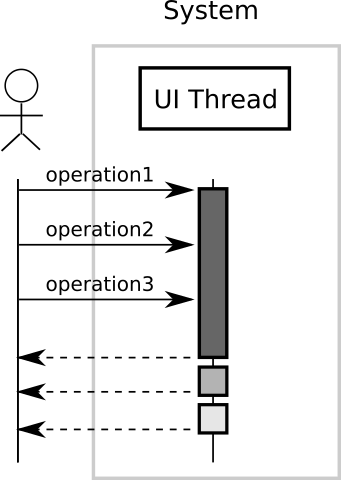
\includegraphics[height=6cm]{asynchrony/sync.png}
\caption{Synchronous}
\label{fig:sync}
\end{subfigure}
\begin{subfigure}{0.4\textwidth}
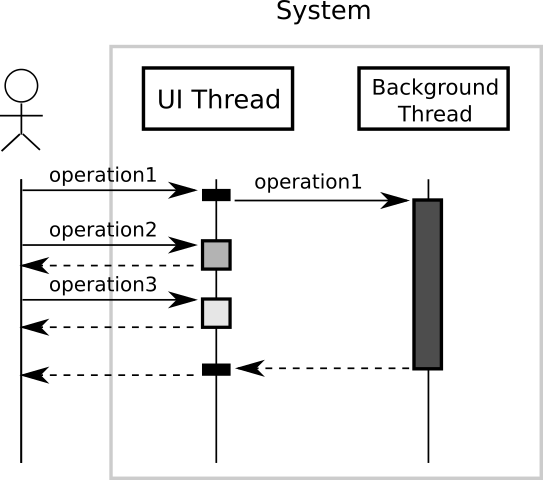
\includegraphics[height=6cm]{asynchrony/async.png}
\caption{Asynchronous}
\label{fig:async}
\end{subfigure}
\end{center}
\caption{Synchronous vs. Asynchronous Execution}
\label{fig:sync-vs-async}
\end{figure}

Listings~\ref{code:asyncRunnableExample} and~\ref{code:asyncFutureExample} are two basic examples of asynchronous implementations in \framework{Java}. The implementation of Listing~\ref{code:asyncRunnableExample} is fire and forget, which means, that no result is expected. The asynchronous operation starts in line 4 and the rest of the code keeps running sequentially, regardless of the amount of time required to finish the asynchronous operation. The implementation of Listing~\ref{code:asyncFutureExample} does return a result. The asynchronous operation starts in line 4 and the result is retrieved in line 9. These examples are used in the next sections to explain the concepts of data races and promises, also called futures.

\begin{center}
\begin{minipage}{0.42\textwidth}
\begin{sourcecode}
\begin{javacode}{}
Runnable runnable = () -> performOpAsync();

Thread thread = new Thread(runnable);
thread.start();

performOperation();
// performOpAsync and performOperation run concurrently
\end{javacode}
\caption{Async Runnable (Fire \& Forget)}
\label{code:asyncRunnableExample}
\end{sourcecode}
\end{minipage}\hspace{0.6cm}
\begin{minipage}{0.53\textwidth}
\begin{sourcecode}
\begin{javacode}{}
Callable<Integer> task = () -> computeResult();

ExecutorService ex = Executors.newFixedThreadPool( 4 );
Future<Integer> future = ex.submit( task );

performOperation();
// computeResult and performOperation run concurrently

Integer asyncResult = future.get();// blocks until task has completed
\end{javacode}
\caption{Async Callable (Future)}
\label{code:asyncFutureExample}
\end{sourcecode}
\end{minipage}
\end{center}

\section{Data Races}
Asynchronous implementations and shared memory models are vulnerable to data races. A data race occurs when multiple threads write a variable in an unspecific order \cite{bookDataRaces}. Since the order in which threads are executed is not well-defined, the result of the modified variable is non-deterministic. To avoid this problem, the developer has to implement locks to make sure that the order of execution is deterministic.

In Listing~\ref{code:asyncRunnableExample} there are two operations that run concurrently, \code{performOpAsync} and \code{performOperation}. Assuming that these methods modify a variable \code{var} and that there is no synchronization mechanism, then we have a data race because we cannot tell for sure which operation modified the value at last. The same happens in Listing~\ref{code:asyncFutureExample} with \code{computeResult} and \code{performOperation}.

\section{Promises}
Promises, also known as Futures, are language constructs that are used to synchronize concurrent code. These constructs consist of a reference to the result of a running operation~\cite{promisesDef}.

In \framework{JavaScript} for example, \framework{Promise}s can be \code{pending} (not started), \code{fulfilled} (successful operation) or \code{rejected} (failed operation) ~\cite{promises}. Since \framework{Promise}s can be chained together, developers need not to use traditional callback-based approaches to handle the return values. According to previous studies, chained calls are easier to understand than callback-based approaches ~\cite{promisesSpring}.

Listing~\ref{code:asyncFutureExample} shows an example of Futures in \framework{Java}. First the \code{task} is executed by the \code{ExecutorService} in a background thread. This call returns the reference to the object that contains the result, in this case, called \code{future}. Then, a second operation called \code{performOperation}, runs in the current thread. After this last operation has completed, we are ready to read the result from the asynchronous task. If the result is not available, then this call waits until the result has been computed. Otherwise, it writes the result in the variable \code{asyncResult} and continues the execution of the next lines of code.

\section{Automated Refactoring}
\label{sec:automated-refactoring}
Refactoring consists of modifying the source code of a program without changing its behavior. Refactoring can be applied to extract a reusable component, improve consistency among components, supporting new features, among others ~\cite{thesisRefactoringFrameworks}. 

Many IDEs already offer refactoring tools. Some of the common refactoring commands are: rename; move; change method signature; extract methods, local variables, constants, interfaces, superclass; among others ~\cite{eclipse, intelliJ}. 

On the other hand, researchers have been developing tools to refactor asynchronous applications. Some of the tools convert synchronous into asynchronous code. Other tools refactor asynchronous code that uses the traditional callback-based approach into method chaining~\cite{paperAsyncMobile, paperStudyRefactoring, thesisJavaScript, paperRetrofittingConcurrency}. We explain these tools in Section~\ref{sec:refactoring-tools}.

\subsection{Abstract Syntax Trees}
Abstract syntax trees (AST), also called syntax trees, are data structures that only contain the essential information about the source code. Parse trees contain additionally the symbols required to compile the code~\cite{bookAST}. Figure~\ref{fig:ast-vs-parser-tree} shows the difference between both types of trees.

\begin{figure}[H]
%\begin{center}
\begin{subfigure}[]{0.4\textwidth}
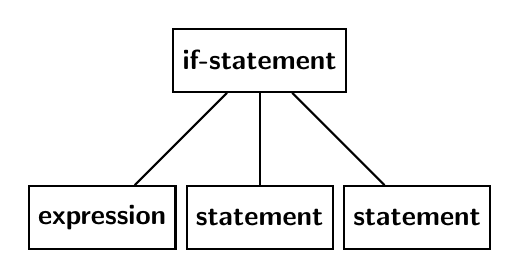
\begin{tikzpicture}[scale=0.5,>=triangle 60,node distance=2cm,thick,
	Edge/.style={-,black,thick},
	ASTNode/.style={rectangle,fill=white,draw=black,font=\sffamily\bfseries,minimum height=0.8cm},
]	
	\node[ASTNode] (A){if-statement};
	\node[ASTNode] (B)[below of=A]{statement};
	\node[ASTNode] (C)[left of=B]{expression};
	\node[ASTNode] (D)[right of=B]{statement};
	
	\path[Edge]
	(A) edge node{}(B)
	(A) edge node{}(C)
	(A) edge node{}(D)
	;
\end{tikzpicture}
\caption{Abstract Syntax Tree}
\label{fig:ast}
\end{subfigure}
%\end{center}
%\begin{center}
\begin{subfigure}[]{0.6\textwidth}
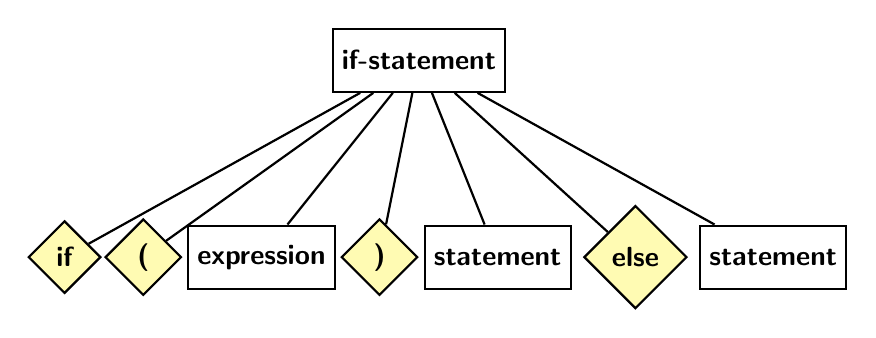
\begin{tikzpicture}[scale=0.5,>=triangle 60,node distance=2cm,thick,
	Edge/.style={-,black,thick},
	ASTNode/.style={rectangle,fill=white,draw=black,font=\sffamily\bfseries,minimum height=0.8cm},
	Symbol/.style={diamond,fill=\myMarkerColor,draw=black,font=\sffamily\bfseries},	
]	
	%\draw[help lines,step=5mm,gray!20] (0,0) grid (18,5);
	\node[ASTNode] (A) at (9,5){if-statement};
	\node[ASTNode] (B) at (11,0){statement};
	\node[Symbol] (C) at (8,0) {)};
	\node[ASTNode] (D)at (5,0) {expression};
	\node[Symbol] (E) at (2,0) {(};
	\node[Symbol] (F) at (0,0) {if};
	\node[Symbol] (G) at (14.5,0) {else};
	\node[ASTNode] (H) at (18,0) {statement};
	
	\path[Edge]
	(A) edge node{}(B)
	(A) edge node{}(C)
	(A) edge node{}(D)
	(A) edge node{}(E)
	(A) edge node{}(F)
	(A) edge node{}(G)
	(A) edge node{}(H)
	;
\end{tikzpicture}
\caption{Parser Tree}
\label{fig:parser-tree}
\end{subfigure}
%\end{center}
\caption{Abstract Syntax Tree vs. Parser Tree ~\cite[p. 216]{bookAST}}
\label{fig:ast-vs-parser-tree}
\end{figure}


As we mentioned in Section~\ref{sec:automated-refactoring}, most IDEs offer refactoring tools. Eclipse, for example, uses AST to get details about the source code and write or modify changes in it (Figure~\ref{fig:ast}).

\section{Functional Programming}
Functional programming is a programming paradigm that uses mathematical functions as its main programming construct~\cite{bookFunctionalProgramming}. This paradigm avoids using concepts such as state and mutable data. Avoiding these concepts facilitates implementation, testing, debugging and code comprehension~\cite{bookFunctionalProgrammingScala}.

In Listings~\ref{code:imperative-pro} and~\ref{code:functional-pro} we compare imperative and functional programming. One can see, that the functional implementation is much compacter than the imperative one. However, this does not apply for every case. Developers must reason about which of these paradigms are more suitable to the given problem.

\begin{center}
\begin{minipage}{0.47\textwidth}
\begin{sourcecode}
\begin{javacode}{}
List<Integer> numbers = 
	Arrays.asList( 1, 3, 4, 5, 8, 13, 15 );
List<String> evenNumbers = new ArrayList<>();
for ( int i = 0; i < numbers.size() ; i++ ) {
    Integer n = numbers.get(i);
    if ( n % 2 == 0)
        evenNumbers.add(String.valueOf(n));
}
doSomething(eventNumbers);
\end{javacode}
\caption{Imperative Programming (Java 8)}
\label{code:imperative-pro}
\end{sourcecode}
\end{minipage}\hspace{0.6cm}
\begin{minipage}{0.47\textwidth}
\begin{sourcecode}
\begin{javacode}{}
List<Integer> numbers = 
	Arrays.asList( 1, 3, 4, 5, 8, 13, 15 );
List<String> eventNumbers = numbers.stream()
        .filter(n -> n % 2 == 0)
        .map(n -> String.valueOf(n))
        .collect(Collectors.toList());
doSomething(eventNumbers);
\end{javacode}
\caption{Functional Programming (Java 8)}
\label{code:functional-pro}
\end{sourcecode}
\end{minipage}
\end{center}

\section{Event Driven Programming}
Event driven programming consists of pieces of code that get executed when an event occurs. Most Windows programs are a good example of this since they are written using event-driven models. If an event never occurs, then the piece of code associated with that event will never be executed. If there is no piece of code associated with an event, then the event will be ignored.~\cite{bookEventDrivenProgramming}.

\subsection{Reactive Programming}
Reactive programming is a programming paradigm that consists in the propagation of change. This programming model is considered a special case of the event-driven paradigm. The events refer mostly to data changes~\cite{bookLearningReactive}. In reactive programming, there is a data-flow graph that indicates how the changes are propagated.
 
Figure~\ref{fig:dataflow} illustrates how reactive programming works. The operation~$a + b$ produces the result~$r$. The first state is: $a=10$, $b=5$, $r=15$. In imperative programming, changing the values of~$a$ and/or~$b$ does not automatically affect the result~$r$, but in reactive programming that is not the case. If the value of~$a$~or~$b$ changes, the operation $+$ is performed and $r$ is updated. 

The previous example also shows a relation between the observer pattern and reactive programming. Let ~$a$ and~$b$ be the subjects and~$r$ be the observer.  If~$r$ updates its value every time~$a$~or~$b$ change, then the behavior described corresponds to a reactive program as well.

\begin{center}
\begin{figure}[h]
\begin{subfigure}{0.5\textwidth}
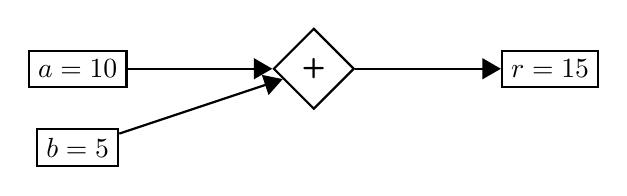
\begin{tikzpicture}[scale=0.7,>=triangle 60,node distance=3cm,thick,
	Edge/.style={->,black,thick},
	Num/.style={rectangle,fill=white,draw=black,font=\sffamily\bfseries},	
	Op/.style={diamond,fill=white,draw=black,font=\sffamily\bfseries},	
	NumberFont/.style={font=\footnotesize},
]	
	\node[Num] (A){$a=10$};
	\node[Num] (B)[below of= A, node distance=1cm]{$b=5$};
	\node[Op] (C)[right of= A]{+};
	\node[Num] (D)[right of= C]{$r=15$};
	
	\path[Edge]
	(A) edge node{}(C)
	(B) edge node{}(C)
	(C) edge node{}(D)
	;
\end{tikzpicture}
\caption{{\bf State 1:} $a=10$, $b=5$, $r=15$}
\end{subfigure}
\begin{subfigure}{0.5\textwidth}
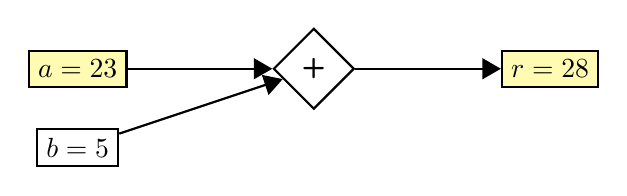
\begin{tikzpicture}[scale=0.7,>=triangle 60,node distance=3cm,thick,
	Edge/.style={->,black,thick},
	Num/.style={rectangle,fill=white,draw=black,font=\sffamily\bfseries},	
	Op/.style={diamond,fill=white,draw=black,font=\sffamily\bfseries},	
	NumberFont/.style={font=\footnotesize},
]	
	
	\node[Num, fill=\myMarkerColor] (A){$a=23$};
	\node[Num] (B)[below of= A, node distance=1cm]{$b=5$};
	\node[Op] (C)[right of= A]{+};
	\node[Num, fill=\myMarkerColor] (D)[right of= C]{$r=28$};
	
	\path[Edge]
	(A) edge node{}(C)
	(B) edge node{}(C)
	(C) edge node{}(D)
	;
\end{tikzpicture}
\caption{{\bf State 2:} $a \rightarrow 23$ then $a=23$, $b=5$, $r=28$}
\end{subfigure}
\caption{Dataflow Example}
\label{fig:dataflow}
\end{figure}
\end{center}

\section{Observer Pattern}
The idea of the observer pattern is to establish a one-to-many relationship between objects. The dependent objects are called observer. The independent objects or subjects notify their observers when their state change. This pattern allows developers modifying observers and subjects independently. Also, observers can be added without applying changes to the existing subject nor the other observers~\cite{bookDesignPatterns}.

The usage of the observer pattern in asynchronous applications can cause backpressure problems when the subject notifies changes faster than the observer's capacity to process them. There are several solutions to tackle this problem. One of them is to have a buffer to accumulate the data received from the subject. Since the buffer can get full, this solution does not work for every case. An alternative solution is to block the notifications from the subject until the data has been processed by the observer~\cite{rxJavaBackpressure}. The disadvantage of the last approach is that the subject is as fast as the slowest observer. A combination of both approaches is also possible.

\section{New Technologies}
Empirical studies have shown that reactive programming increases the correctness of program comprehension without requiring neither more time to analyze the program nor advance programming skills~\cite{paperReactiveComprehension}. Furthermore, there are new technologies that are based on event-driven programming models and reactivity. \framework{Flapjax}, \framework{ReactiveX} and \framework{Agera} are some of them. These technologies also agree that reactive and event-driven approaches simplify code writing and comprehension~\cite{agera, reactiveX, paperFlapjax}.

\subsection{Flapjax}
\framework{Flapjax} is a language built on top of \framework{JavaScript} to enable event-driven programming. 
It can also be used as a library if developers do not want to use the Flapjax-to-JavaScript compiler~\cite{paperFlapjax}.

\framework{Flapjax} introduces two new data types, \code{Behavior}s and \code{Event-Stream}s. \code{Behavior}s are values that change over time  (i.e: a variable). Changes in \code{Behavior}s propagate automatically, facilitating developers consistency in their applications. \code{Event-Stream}s represent the input sources.~\cite{paperFlapjax}.

Listing~\ref{code:javaScript} shows a basic \framework{JavaScript} example where a string value \code{id="validationMessage"} (line~31) is updated when an event \code{"onChange"} is triggered. Since there is no native \framework{JavaScript} call to determine if an input have changed, a possible (trivial) implementation could be for example triggering the \code{validateNumber} function every $200ms$ (line~22). We chose this time interval because we consider it small enough to be perceived as an immediate change. Notice that the function \code{startValidation} must be called on load (line~27). The validation logic is implemented in the function \code{validateNumber} (line~5).

Listing~\ref{code:flapjax} shows the same example using \framework{Flapjax}. In this case, \framework{Flapjax} was downloaded and used as a library (line~2). The implementation basically defines a behavior for the input \code{numb} (line~7). The function \code{liftB} (line~8) creates a time varying value which is used for updating the \code{validationMessage}. The function \code{loader} defines the events (line~8) and their reaction (line~20). This function is also called on load (line~26). This example shows how \framework{Flapjax} allows keeping the UI consistency without having to implement a mechanism for updating a particular field. Instead, events and reaction to those events are defined.

More interactive examples can be found at \framework{Flapjax}'s official site~\cite{urlFlapjaxDemo}.

\code{Event-Stream}s can be processed in \framework{Flapjax} using functions such as: \code{mapE}, \code{mergeE}, \code{filterE}, \code{andE}, \code{orE}, \code{notE}, among others.

These functions are also available in \framework{ReactiveX}~\cite{reactiveX}.

\begin{figure}[]
\begin{minipage}{0.48\textwidth}
\begin{sourcecode}
\begin{minted}[tabsize=2,frame=lines,framesep=2mm,rulecolor=\color{black!10},linenos,frame=single,fontsize=\small, breaklines=true,highlightcolor=\myMarkerColor, highlightlines={5,22,27,31}]{html}
<html>
<head>
<title>JavaScript</title>
<script type="text/javascript">
function validateNumber() {
    var x, text;
    x = document.getElementById("numb").value;
    if ( x == ""){
            text = "";
    } else if (isNaN(x)) {
        text = "Not a number";
    } else if (x < 1 || x > 10) {
        text = "Number out of Range";
    } else {
        text = "Valid number";
    }
    document.getElementById("validationMessage")
    	.innerHTML = text;
}
function startValidation(){
  validation = 
  		setInterval("validateNumber()",  200);
}
</script>
</head>

<body onload="startValidation()">
<h1>Number Validator (JavaScript)</h1>
<p>Please input a number between 1 and 10:</p>
<input id="numb">
<p id="validationMessage"></p>
</body>
</html>
\end{minted}

\caption{JavaScript}
\label{code:javaScript}
\end{sourcecode}
\end{minipage}\hspace{0.75cm}
\begin{minipage}{0.49\textwidth}
\begin{sourcecode}
\begin{minted}[tabsize=2,frame=lines,framesep=2mm,rulecolor=\color{black!10},linenos,frame=single,fontsize=\footnotesize, breaklines=true,highlightcolor=\myMarkerColor, highlightlines={2,7-8,20,26,30}]{html}
<html>
<script type="text/javascript" src="flapjaxLibrary.js"></script>
<title>Flapjax</title>
<script type="text/javascript">

function loader() {
  var valB = extractValueB('numb', 'value');
  var validationStrB = valB.liftB(
    function (s) {
      if ( s == ""){
          return "";
      } else if (isNaN(s)) {
          return "Not a number";
      } else if (s < 1 || s > 10) {
          return "Number out of Range";
      } else {
          return "Valid number";
      }
    });
  insertDomB(validationStrB, 'validationMessage');
}

</script>
</head>

<body onload="loader()">
<h1>Number Validator (Flapjax)</h1>
<p>Please input a number between 1 and 10:</p>
<input id="numb">
<p id="validationMessage"></p>
</body>
</html>
\end{minted}

\caption{Flapjax}
\label{code:flapjax}
\end{sourcecode}
\end{minipage}
\end{figure}


\subsection{ReactiveX}
\framework{ReactiveX} is a library that supports data streams and reactivity. It is available in many platforms (\framework{Java}, \framework{JavaScript}, \framework{C\#}, \framework{C++}, \framework{Ruby}, \framework{Android}, among others)~\cite{reactiveX}. 

\begin{figure}[]
\begin{sourcecode}
\begin{javacode}{4,12,15}
...
List<Product> existingProducts = new ArrayList<>();
	existingProducts.addAll(productDao.getProducts());
	Observable.from(existingProducts)
		.filter(p -> 
					p.getPrice() > 50 && 
					p.getStore().equals(STORE_A))
		.map(p -> new Product(
						p.getId(), 
						p.getPrice() * 1.10, 
						STORE_B))
		.subscribeOn(Schedulers.computation()) // do in background
		.doOnNext(p -> productDao.save(p))
		.doOnError(t -> handleError(t))
		.observeOn(Schedulers.uiThread()) // only as example: this scheduler doesn't exist
		.doOnCompleted(() -> updateUI())
		.subscribe();
	);
...
\end{javacode}
\caption{RxJava: Streams}
\label{code:rxJava-streams}
\end{sourcecode}
\end{figure}

The API of \framework{ReactiveX} for \framework{Java} programs is called \framework{RxJava}. By using \framework{RxJava} it is possible to write asynchronous programs in a functional fashion. Additionally, since \framework{RxJava} is based on the observer pattern, it is also possible to implement reactive models.

Listing~\ref{code:rxJava-streams} shows an example where we use \framework{RxJava} to select some items, transform them and save the newly generated items. We use a background thread for the operations and update the UI when done. The process is as follows: First, we create a \code{rx.Observable} object using the method \code{Observable.from} (line~4). Then, we invoke further methods to modify the data stream (\code{filter}, \code{map}). After that, we specify in which thread the operation must be executed (line~12). RxJava offers several \code{Scheduluer}s for that purpose. However, one can also use custom executors. Next, we define the save operation using \code{doOnNext} (line~13). Since in this example the \code{doOnCompleted} operation must be executed in the UI thread, we place the \code{observeOn} declaration before \code{doOnCompleted} (line~15). Finally, we subscribe the observable. This subscription starts executing the async operation.

\begin{figure}[t]
\begin{sourcecode}
\begin{javacode}{8,11,14}
public static void main( String[] ars ) {
    BehaviorSubject<Integer> a = BehaviorSubject.create( 1 );
    BehaviorSubject<Integer> b = BehaviorSubject.create( 2 );
    final BehaviorSubject<Integer> sum = BehaviorSubject.create( 0 );
    final BehaviorSubject<Integer> mult = BehaviorSubject.create( 0 );
    Observable.combineLatest( a, b, ( n1, n2 ) -> n1 + n2 ).subscribe( sum );
    Observable.combineLatest( a, b, ( n1, n2 ) -> n1 * n2 ).subscribe( mult );
    // check initial states of sum and mult
    System.out.println(sum.getValue()); // output: 3
    System.out.println(mult.getValue()); // output: 2
    a.onNext(5); // modifies subject a
    System.out.println(sum.getValue()); // output: 7
    System.out.println(mult.getValue()); // output: 10
    b.onNext(10); // modifies subject b
    System.out.println(sum.getValue()); // output: 15
    System.out.println(mult.getValue()); // output: 50
}
\end{javacode}
\caption{RxJava: Reactive Code}
\label{code:rxJava-reactive-code}
\end{sourcecode}
\end{figure}

Listing~\ref{code:rxJava-reactive-code} shows an example where we use \framework{RxJava} to implement two reactive operations (addition and multiplication). The first step is to define the subjects (lines 2-3). Then, we declare the subscribers (lines 4-5), also called observers. Finally, we define the behavior (lines 6-7). We do this by creating an observable that combines both subjects and defines the result. Then we subscribe the corresponding subscriber to each observable. Lines 11 and 14 show how we manipulate the subjects, so the changes are propagated to the subscribers.

\framework{RxJava} offers many other classes and methods for building asynchronous reactive models. Explaining all of them does not belong to the scope of this thesis. More information and examples about this library can be found at~\cite{bookLearningReactive}.

\subsection{Java 8}
\framework{Java 8} introduces a series of classes that allows working with data streams in a functional fashion~\cite{bookJava8Streams}. However, in contrast to \framework{RxJava}, the new classes of \framework{Java 8} do not support defining which operations should be executed in the background and which ones on the UI thread.

\begin{figure}[h]
\begin{minipage}{0.48\textwidth}
\begin{sourcecode}
\begin{javacode}{2-8,10,14}
Observable.from(productDao.getProducts())
        .filter(p ->
                p.getPrice() > 50 &&
                p.getStore().equals(STORE_A))
        .map(p -> new Product(
                p.getId(),
                p.getPrice() * 1.10,
                STORE_B))
        .subscribeOn(Schedulers.computation())
        .doOnNext(p -> productDao.save(p))
        .doOnError(t -> handleError(t))
        .observeOn(Schedulers.uiThread()) // only as example: this scheduler doesn't exist
        .doOnCompleted(() -> updateUI())
        .subscribe();
\end{javacode}
\caption{RxJava (Products Example)}
\label{code:rxJava-compared}
\end{sourcecode}
\end{minipage}\hspace{0.7cm}
\begin{minipage}{0.48\textwidth}
\begin{sourcecode}
\begin{javacode}{2-9}
productDao.getProducts().stream()
        .filter(p ->
                p.getPrice() > 50 &&
                p.getStore().equals(STORE_A))
        .map(p -> new Product(
                p.getId(),
                p.getPrice() * 1.10,
                STORE_B))
        .forEach(p -> productDao.save(p));
\end{javacode}
\caption{Java 8 (Products Example)}
\label{code:java8-compared}
\end{sourcecode}
\end{minipage}
\end{figure}

Listings~\ref{code:rxJava-compared} and~\ref{code:java8-compared} show a comparison between \framework{RxJava} and \framework{Java 8}. There are two method invocations that are identical and one invocation that is similar but not completely equivalent. Using functions such as \code{filter} and \code{map} can be done with both, \framework{RxJava} and \framework{Java 8}, in the same way. The call \code{doOnNext} is similar to \code{forEach} in the sense of iterating through all items and doing some operations with them. The big difference is that \code{forEach} actually starts executing the operation while \code{doOnNext} only defines it. In the second case the operation starts when the observable is subscribed (Listing~\ref{code:java8-compared}, line 14). Also, \code{forEach} does not not allow chaining futher methods. Methods such as \code{subscribeOn}, \code{doOnError}, \code{observeOn}, \code{doOnCompleted}, among others have no equivalent in \framework{Java 8}.

\section{Async Constructs}
There are several async constructs in many different frameworks and platforms. We want to focus particularly in \code{SwingWorker}s because that is the construct that we analyze in this thesis. Additionally, we want to explain the basics about \code{AsyncTask}s because previous research has been analyzing them and developing refactoring tools for different purposes.

Figure~\ref{fig:asynctask-execution} illustrates in which threads the methods of an \code{AsyncTask} are executed. In this example, the \code{AsyncTask} starts with the invocation of \code{execute}. Then \code{onPreExecute} is invoked in the UI thread. As soon as this method finishes, \code{doInBackground} is invoked on a background thread. While the asynchronous operation is running, data can be sent to UI thread throw the invocation of \code{publish}. This data is processed in the UI thread using the logic specified in \code{onProgressUpdate}. The \code{publish} method can be invoked multiple times. Finally, when the asynchronous operation has completed, the result is processed in the UI thread using the \code{onPostExecute} method.

Figure~\ref{fig:swingWorker-execution} shows which methods of a \code{SwingWorker} are executed in the background and which ones in the UI thread. The \code{SwingWorker} also starts when \code{execute} is invoked. Notice that \code{SwingWorker}s do not have an \code{onPreExecute} method. Like \code{AsyncTask}s, \code{SwingWorker}s also have a \code{publish} method to send data to the UI thread. This data is processed according to the logic contained in the \code{process} method. The \code{publish} method can be called multiple times too. Finally, after the asynchronous operation has completed, the method \code{done} is invoked, which is also executed in the UI thread. Inside \code{done} the method \code{get} can be invoked, in order to have access to the result of the async operation.

\begin{figure}[h]
\begin{subfigure}{0.5\textwidth}
\begin{center}
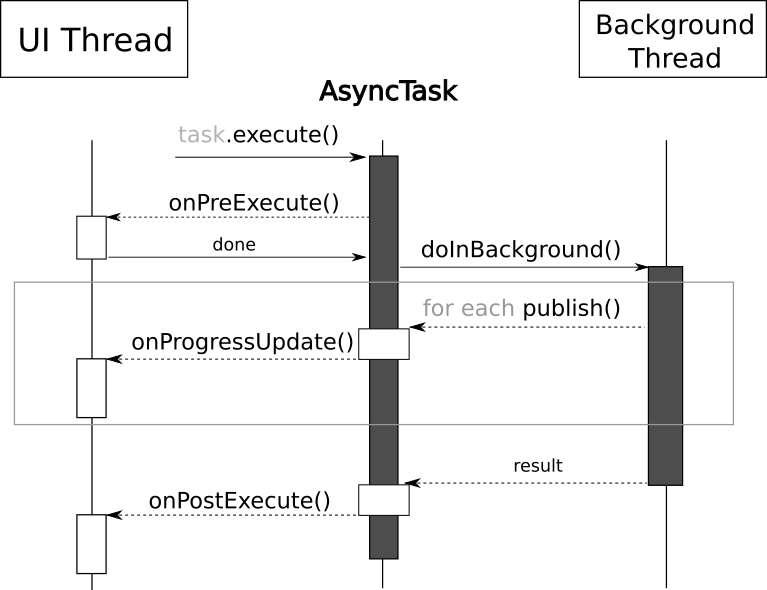
\includegraphics[height=6.5cm]{async-constructs/asynctask.png}
\end{center}
\caption{AsyncTask Execution}
\label{fig:asynctask-execution}
\end{subfigure}
\begin{subfigure}{0.5\textwidth}
\begin{center}
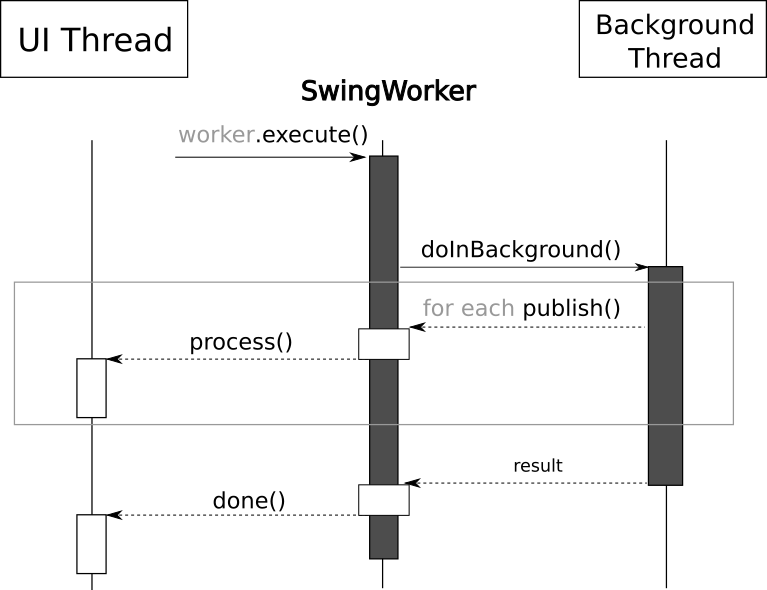
\includegraphics[height=6.5cm]{async-constructs/swingworker.png}
\end{center}
\caption{SwingWorker Execution}
\label{fig:swingWorker-execution}
\end{subfigure}
\caption{AsyncTask vs. SwingWorker}
\end{figure}

\code{SwingWorker}s and \code{AsyncTask}s also have some similar methods. We match these methods in Table~\ref{table:worker-task-equivalent}. Methods written in {\bf bold} depend on the state of the \code{SwingWorker} and/or \code{AsyncTask}.

\begin{table}[h]
{\small
\begin{center}
\begin{tabular}{|C{6cm} | C{6cm}|}
\hline
\bf SwingWorker~\cite{swingworkerapi} & \bf AsyncTask~\cite{ulrAndroidAsyncTask}\\\hline
doInBackground() & doInBackground(...)\\
process(...) & onProgressUpdate(...)\\
publish(...) & publishProgress(...)\\
done() & onPostExecute(...)\\\hline
cancel(...) & cancel(...)\\
execute() & execute(...)\\
\bf getState() & \bf getStatus()\\
\bf isCancelled() & \bf isCancelled()\\
get() & get() \\
get(...) & get(...)\\\hline
\end{tabular}
\end{center}
\caption{Equivalent Methods - SwingWorker vs. AsyncTask (1)}
\label{table:worker-task-equivalent}
}
\end{table}

However, not all methods have an equivalent. Table~\ref{table:worker-task-non-equivalent} shows all methods that do not have a match. Again, methods written in {\bf bold} depend on the state of the class. As we can see, \code{SwingWorker}s have more methods that depend on the state than \code{AsyncTask}s. This point will be discussed again in Chapter~\ref{chapter:design}, when we talk about the refactoring approach that we use to convert \code{SwingWorker}s into \framework{RxJava}.

\begin{table}[h]
{\small
\begin{center}
\begin{tabular}{|C{6cm} | C{6cm}|}
\hline
\bf SwingWorker~\cite{swingworkerapi} & \bf AsyncTask~\cite{ulrAndroidAsyncTask}\\\hline
\bf addPropertyChangeListener(...) & --\\
\bf firePropertyChange(...) & --\\
\bf getProgress() & --\\
\bf getPropertyChangeSupport() & --\\
\bf isDone() & --\\
\bf removePropertyChangeListener(...)& --\\
run()& --\\
\bf setProgress(...)& --\\\hline
-- & onPreExecute() \\
-- & executeOnExecutor(...)\\
-- & onCancelled()\\\hline
\end{tabular}
\end{center}
\caption{Equivalent Methods - SwingWorker vs. AsyncTask (2)}
\label{table:worker-task-non-equivalent}
}
\end{table}

For more details about the \code{SwingWorker} API go to Appendix~\ref{swingworkerapi}. 

\section{Refactoring Tools}
\label{sec:refactoring-tools}
Modern programming languages such as \framework{C\#}, \framework{Visual Basic}, \framework{F\#} and \framework{Scala} have introduced \code{asycn} constructs and \code{await} calls to facilitate the implementation of asynchrony. With these constructs developers do not need to implement callbacks to manage asynchrony \cite{paperAsyncMobile}. 

According to previous studies, async constructs are being underused or misused. A common example of misused asynchrony is to introduce elements that appear to be asynchronous, but due to semantic mistakes, the code still runs synchronously. To tackle this problem, refactoring tools have been developed~\cite{paperAsyncMobile}. 

Refactoring asynchronous applications is not trivial. Therefore researchers have already started developing tools to assist developers in this task. These tools can be classified into three groups:

\begin{enumerate}
	\item Synchronous code $\rightarrow$ asynchronous code
	\item Callback based asynchronous code $\rightarrow$ method chained asynchronous code
	\item Correction of anti-patterns and performance improvements
\end{enumerate}

\subsection{Synchronous $\rightarrow$ Asynchronous}
Refactoring synchronous \framework{Android} applications to be asynchronous is not an easy task. According to a previous research, the reason of this might be that most documentation focuses on the design from scratch rather than on the process of converting existing synchronous code into asynchronous. They also state that there are not enough methods neither tools for this kind of refactoring~\cite{paperAsyncMobile}.

Motivated by these facts, they developed \textsc{Asynchronizer}. \textsc{Asynchronizer} targets \framework{Android} applications. It can be used to convert synchronous code into asynchronous by using an \code{AsyncTask}~\cite{paperRetrofittingConcurrency}. \textsc{Asynchronizer} basically moves the synchronous code into the \code{doInBackground} method of the \code{AsyncTask}. Then it analyzes the rest of the code in order to determine which part can be placed into the \code{onPostExecute} handler. Finally, it creates an instance of the class in the main thread and calls its \code{execute} method.

Converting synchronous code into asynchronous might produce data races. To make sure that there are no data races after refactoring, they implemented an extension of the \textsc{IteRace} detector. This component is included with \textsc{Asynchronizer}. It is important to mention that this check does not run automatically. Developers have to explicitly check for data races after refactoring the code. Reported data races should be analyzed by developers to determine whether they are real or fake. To do that, developers must consider the application's workflow. Some methods in \framework{Android} are by design never called concurrently (.i.e \code{onCreateView} and \code{onDestroyView})~\cite{paperRetrofittingConcurrency}.

\subsection{Callback based $\rightarrow$ Method chained}
\textsc{Asyncifier} is a \framework{.NET} tool that automatically refactors callback-based asynchronous code into \code{async/await}. This tool has already been tested using real-world applications~\cite{paperAsyncMobile}.

Another tool in this category is \textsc{PromisesLand}. This tool converts \framework{JavaScript} asynchronous callbacks into \framework{Promises}. This refactoring facilitates code comprehension by replacing callbacks with chained calls~\cite{thesisJavaScript}. \textsc{PromisesLand} consist of a static analyzer and a transformation engine. The static analyzer is in charge of searching for asynchronous patterns that can be refactored into \framework{Promises}. The transformation engine is responsible for performing the refactoring~\cite{thesisJavaScript}.

In the last months, \textsc{RxFactor} was developed. As we mentioned before, this tool has some similarities with \toolcore{}. \textsc{RxFactor} takes the code from \code{AsyncTask}s and generates a functional implementation of that code using the \framework{ReactiveX} API. Although \textsc{RxFactor} and our tool have the same goal, and \code{AsyncTask}s are very similar to \code{SwingWorker}s, the refactoring approaches used are very different. We compare both approaches in Chapter~\ref{chapter:design}.

\subsection{Anti-patterns $\rightarrow$ Improvements}
\code{AsyncTask} should only be used for short-running operations (approx. less than a second). For long-running operations the class \code{IntentService} should be used ~\cite{paperStudyRefactoring}. This refactoring is also not trivial. According to a previous research, this might be due to the developer's lack of knowledge about how to use this class. The author of that study believes that the lack of knowledge is the consequence of not having enough production-level examples that use \code{IntentService}~\cite{paperStudyRefactoring}. \textsc{AsyncDroid} is a tool that can be used to convert \code{AsycnTask} into \code{IntentService}.

\textsc{AsyncFixer} is a \framework{.NET} tool that can be used to recognize performance anti-patterns of \java{async/await} in mobile applications (i.e. in \framework{Windows Phone}). This tool also suggests fixes. \textsc{AsyncFixer} has already been successfully tested using real-world applications~\cite{paperAsyncMobile}.

\chapter{Design of the System}
\label{chapter:design}

Previous studies show that functional and reactive programming models improve code writing and code comprehension~\cite{promises, paperReactiveComprehension}. In this thesis, we propose an approach to refactor \code{SwingWorker}s into \framework{RxJava}. This refactoring enables a series of methods that can be used to implement reactive models in a functional fashion. Basically, the process starts by using \toolextension{}, a tool that we developed to perform the \code{SwingWorker} to \framework{RxJava} transformation automatically. Then developers can use the methods available in \framework{RxJava} to build their reactive models.

\section{Use Case Example}

The next example illustrates how the process works. The example bases on \framework{Juneiform} (Figure~\ref{fig:juneiform}), an application with OCR that extracts text from images.

\begin{figure}[h]
\begin{center}
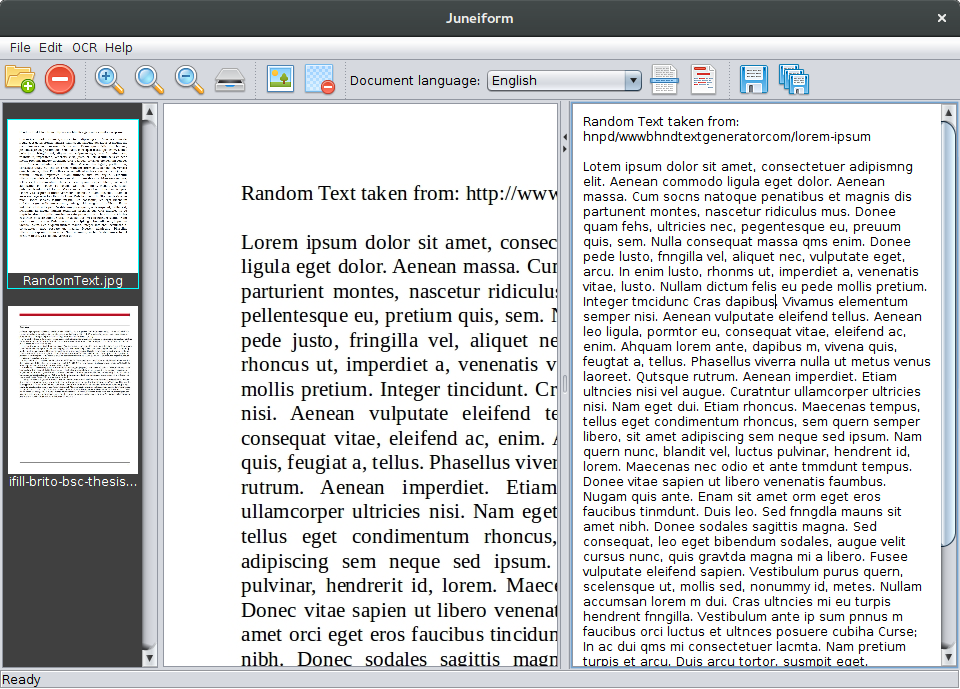
\includegraphics[width=0.95\textwidth]{juneiform/Juneiform.png}
\caption{Juneiform: \url{https://bitbucket.org/Stepuk/juneiform}\\\href{https://bitbucket.org/Stepuk/juneiform/src/c07e0bbcf17c2d63137f28109cf5812a231692de?at=default}{c07e0bbcf17c2d63137f28109cf5812a231692de}}
\label{fig:juneiform}
\end{center}
\end{figure}

In this example we focus on two classes, \code{DocumentLoader} and \code{Editor}. The \code{DocumentLoader} is the class in charge of importing the images into \framework{Juneiform}. Here we want to extend the functionality to add four observers to the event ``load document''. The \code{Editor} class is in charge of performing the OCR. Here we want to display a loading spinner and close it after the optical character recognition has completed. Furthermore, the output text is copied automatically to the clipboard.

\subsection{DocumentLoader}
The original implementation of \code{DocumentLoader} waits until all images are loaded before showing them in the UI. Since we want to work with streams, we slightly modified the original source code, so that the images are displayed one by one, as soon as they are available.

Listings~\ref{code:example-original} and~\ref{code:example-refactored} show the source code before and after refactoring  the class \code{DocumentLoader} with \toolextension{}. The differences in both code snippets are highlighted. We modified the source code in these snippets to spare a few lines. The method \code{createDocument} does not exist in the original code, but it allows us to write the same logic using fewer lines. As one can see, the code did not change much, but now we are using subscribers and observables. 

\begin{figure}[h]
\begin{minipage}{0.45\textwidth}
\begin{sourcecode}
\begin{javacode}{2,6}
public abstract class DocumentLoader 
	extends SwingWorker<List<Document>, Document> {
    ...
    public void load(File... files) {
        this.files = files;
        execute();
    }

    protected List<Document> doInBackground() 
    	throws Exception {
        ...
        publish(new Document(...
        ...
    }

    protected void process(List<Document> chunks){
        fetchResult( chunks );
    }
    ...
\end{javacode}
\caption{DocumentLoader - Modified Code}
\label{code:example-original}
\end{sourcecode}
\end{minipage}\hspace{0.7cm}
\begin{minipage}{0.51\textwidth}
\begin{sourcecode}
\begin{javacode}{2,6,9-12,19}
public abstract class DocumentLoader 
	extends SWSubscriber<List<Document>, Document> {
    ... 
    public void load(File... files) {
        this.files = files;
        executeObservable();
    }

    private rx.Observable<SWChannel<List<Document>, Void>> 
    	getRxObservable() {
				return rx.Observable.fromEmitter(
				new SWEmitter<List<Document>, Void>() {
				protected List<Document> doInBackground() 
					throws Exception {
				        ...
				        publish(new Document(...
				        ...
				}
			}, Emitter.BackpressureMode.BUFFER);
	}
	protected void process( List<Document> chunks ){
		fetchResult( chunks );
	}
	...
\end{javacode}
\caption{DocumentLoader - Automatically Refactored Code}
\label{code:example-refactored}
\end{sourcecode}
\end{minipage}
\end{figure}

Listings~\ref{code:example-edited} shows how the refactored code can be manually modified to change the behavior of the program using functional and reactive paradigms. In this example, we specify through a filter that only \code{jpg} files should be considered (lines~23-24). Notice that we use functional programming for this. Then we built a reactive model for the files to be imported. Lines~5~to~8 shows how to initialize the \code{Observable}. We want to have a \code{ConnectableObservable} that is executed in the background (\code{Schedulers.computation}) and which observers are executed on the UI thread (\code{SwingScheduler.getInstance}). Then we can register the subscribers (lines 11-14), also called observers. The first observer is in charge of loading the images into \framework{Juneiform}. The next 3 observers only print a string to the console (Listing~\ref{code:example-console}). Notice that these operations are executed in the UI thread. In \framework{Swing} applications the UI thread is called \framework{AWT-EventQueue}. Finally, the \code{ConnectableObservable} must be connected. As a result, we obtain the reactive model described in lines 4 to 17.

\begin{figure}[H]
\begin{sourcecode}
\begin{textcode}{}
[ AWT-EventQueue-0 ] 0 - Updating UI: RANDOMTEXT
[ AWT-EventQueue-0 ] 1 - RANDOMTEXT
[ AWT-EventQueue-0 ] 2 - RANDOMTEXT
[ AWT-EventQueue-0 ] 3 - RANDOMTEXT
[ AWT-EventQueue-0 ] 0 - Updating UI: IFILL-BRITO-BSC-THESIS
[ AWT-EventQueue-0 ] 1 - IFILL-BRITO-BSC-THESIS
[ AWT-EventQueue-0 ] 2 - IFILL-BRITO-BSC-THESIS
[ AWT-EventQueue-0 ] 3 - IFILL-BRITO-BSC-THESIS
\end{textcode}
\caption{Juneiform - Console output after refactoring manually}
\label{code:example-console}
\end{sourcecode}
\end{figure}

\begin{figure}[H]
\begin{sourcecode}
\begin{javacode}{4,10,16,23-25}
...
	public void load( File... files ) {
		this.files = files;
		// setup subject
		ConnectableObservable<SWPackage<List<Document>, Document>> connectableObservable = getRxObservable()
				.observeOn( SwingScheduler.getInstance() )
				.subscribeOn( Schedulers.computation() )
				.publish();
				
		// register subscribers
		connectableObservable.subscribe( swPackage -> fetchResult( swPackage.getChunks() ));
		connectableObservable.subscribe( swPackage -> printChunks( "1", swPackage ));
		connectableObservable.subscribe( swPackage -> printChunks( "2", swPackage ));
		connectableObservable.subscribe( swPackage -> printChunks( "3", swPackage ));
		
		// connect subject with subscribers
		connectObservable( connectableObservable );
	}
	
	private rx.Observable<SWPackage<List<Document>, Document>> getRxObservable() {
		return rx.Observable.fromEmitter( new SWEmitter<List<Document>, Document>(){...
		}, Emitter.BackpressureMode.BUFFER )
				.filter( swPackage -> {
					List<Document> docs = swPackage.getChunks();
					return swPackage.getResult() == null && !docs.isEmpty() && docs.get(0).getName().contains( ".jpg" );
				} );
	}
...
\end{javacode}
\caption{DocumentLoader Class manually modified after \toolextension{}-Refactoring}
\label{code:example-edited}
\end{sourcecode}
\end{figure}


\subsection{Editor}

Similarly, \toolextension{} refactored the class \code{Editor}. After performing the refactoring, one can modify the source code manually to add new features. In this case, we implemented a \code{Util} class for showing and closing a loading spinner. Additionally, we added a method to copy the result of the OCR to the clipboard. Once we have implemented these methods, we can add to the new observable in a functional fashion, as shown in Listing~\ref{code:example-editor} (Lines 6-8). When the observable is subscribed, the loading spinner is shown (\code{doOnSubscribed}). The last emission corresponds to the result. This result is copied to the clipboard using \code{doOnNext}. Finally, the loading spinner is hidden \code{doOnCompleted}. This time we added events using a functional notation.

\begin{figure}[H]
\begin{sourcecode}
\begin{javacode}{6-8}
public class Editor implements ViewInteractor
{
...
		rx.Observable<SWPackage<String, Void>> rxObservable = Observable.fromEmitter( new SWEmitter<String, Void>(){...
		}, Emitter.BackpressureMode.BUFFER )
                .doOnSubscribe( () -> Utils.showLoadingSpinner() )
                .doOnNext( swPackage -> copyToClipBoard( swPackage.getResult() ) )
                .doOnCompleted( () -> Utils.closeLoadingSpinner() );
...
}
\end{javacode}
\caption{Editor Class manually modified after \toolextension{}-Refactoring}
\label{code:example-editor}
\end{sourcecode}
\end{figure}

\section{Refactoring Approach}
As we mentioned before \textsc{RxFactor} and \toolextension{} refactor similar asynchronous constructs. In this section, we show the general idea of the refactoring approach of \textsc{RxFactor} and explain the reason why we decided to use a different one. After that, we present the approach used by our tool.

\subsection{RxFactor Approach}
Listings~\ref{code:rxfactor-before} and~\ref{code:rxfactor-after} summarize how \textsc{RxFactor} refactors \code{AsyncTask}s into \framework{RxJava}. First an \code{Observable} is created by using \code{Observable.fromCallable} (L~\ref{code:rxfactor-after}:~line~14). The argument of this method is a \code{Callable} object, which defines the asynchronous operation. Therefore the routine from \code{doInBackground} (L~\ref{code:rxfactor-before}:~lines~5-7) is written here. 

The \code{publish} (L~\ref{code:rxfactor-before}:~line~7) method cannot be copied inside of \code{fromCallable}, because this method is not defined in objects of type \code{Callable}. To be able to refactor \code{publish} invocations, a \code{Subscriber} is needed. This \code{Subscriber} is obtained from the method \code{getRxUpdateSubscriber} (L~\ref{code:rxfactor-after}:~line 1), where \code{onNext} (L~\ref{code:rxfactor-after}:~line 5) is implemented. As we can see, \code{Subscriber.onNext} and \code{onProgressUpdate} (L~\ref{code:rxfactor-before}:~line 13) are equivalent. 

Since \code{fromCallable} returns a single result, \code{doOnNext} (L~\ref{code:rxfactor-after}:~line~27) is used to read the only and therefore final emission of the observable, which corresponds to the result from \code{doInBackground}. The \code{AsyncTask} processes this result in \code{onPostExecute} (L~\ref{code:rxfactor-before}:~line 19), which is why we find the same piece of code in \code{doOnNext}.


\begin{figure}[h]
\begin{minipage}{0.48\textwidth}
\begin{sourcecode}
\begin{javacode}{2,7,13,19}
new AsyncTask<InputT, PublishT, ResultT>(){
	protected ResultT doInBackground(InputT... params){
		...
		for (...; ...; ...){
			PublishT p = longRunningOperation(...);
			...
			publish(p);
		}
		...
		return result;
	}
	
	protected onProgressUpdate(PublishT... values){
		...
		process(values);
		...
	}
	
	protected void onPostExecute(ResultT result){
		...
		finishTask(result);
		...
	}
}.execute();
\end{javacode}
\caption{Before Refactoring with \textsc{RxFactor}}
\label{code:rxfactor-before}
\end{sourcecode}
\end{minipage}\hspace{0.7cm}
\begin{minipage}{0.48\textwidth}
\begin{sourcecode}
\begin{javacode}{5,15,20,28}
private Subscriber<PublishT> getRxUpdateSubscriber() {
	return new Subscriber<PublishT[]>(){
		public void onCompleted(){ }		
		public void onError(Throwable t) { }		
		public void onNext(PublishT[] values){
			...
			process(values);
			...
		}
	}
}
...

Observable.fromCallable(new Callable<ResultT>() {
	public ResultT call() throws Exception{
		...
		for (...; ...; ...){
			Publish p = longRunningOperation(...);
			...
			getRxUpdateSubscriber().onNext(p);
		}
		...
		return result;
	}
}).subscribeOn(Schedulers.computation())
  .observeOn(AndroidSchedulers.mainThread())
  .doOnNext(new Action1<ResultT>(){
  	public void call(ResultT result) {
		...
		finishTask(result);
		...
  	}
}).subscribe();
\end{javacode}
\caption{After Refactoring with \textsc{RxFactor}}
\label{code:rxfactor-after}
\end{sourcecode}
\end{minipage}
\end{figure}

This refactoring approach is able to transform \code{AsyncTask}s into \framework{RxJava}, as long as the methods \code{getStatus} and \code{isCancelled} are not invoked. The method \code{getStatus} cannot be adapted, because this requires keeping track of the current state, which is not possible in this implementation without adding a helper class or a similar structure. Due to the same reason, the method \code{isCancelled} can also not be refactored. \framework{RxJava} offers a call to determine whether a \code{Subscription} is subscribed or not (\code{isSubscribed}), but this method returns \code{false} if the \code{Observable} has not been subscribed yet, while \code{isCancelled} returns true, when the \code{AsyncTask}s has not started. 

This approach is not suitable for \code{SwingWorker}s because nine out of eighteen methods available in the \code{SwingWorker} API require knowledge of the current state. This was the main reason for us to not use this approach.

There are also other drawbacks about the approach used in \textsc{RxFactor}. Since \code{Observable.fromCallable} is used, only one item is generated by the \code{Observable}. This item is the result of the asynchronous operation. If we connect the \code{Observable} to multiple \code{Subscriber}s, then these observers will only get the final result. Information about the data that was originally processed in the \code{AsyncTask} through \code{onProgressUpdate} will still depend on the \code{Subscriber} that is directly specified in the \code{Observable} (L~\ref{code:rxfactor-after}:~line~21).

Another problem of \textsc{RxFactor} is backpressure. The \code{Subscriber} (L~\ref{code:rxfactor-after}:~lines 5-9) used for publishing intermediate results and the \code{Observable} are totally independent. If the algorithm defined by the \code{Callable} object of the \code{Observable} generates items faster than the time required by the \code{Subscriber} to consume them, then some of these items will be lost and remain unprocessed.

The last disadvantage that we found about the approach used in \textsc{RxFactor} is that two objects from \framework{RxJava} are needed to refactor the public method invocations from the \code{AsyncTask}. Table~\ref{table:asynctask-rx-methods} shows these objects. Basically, most methods can be refactored using \code{rx.Observable}. However, if \code{cancel} is invoked, then one needs to generate a \code{Subscription} from the \code{Observable} and call \code{unsubscribe}.

\begin{table}[H]
\begin{center}
\begin{tabular}{|C{4cm}|C{4cm}|C{4cm}|}
\hline
\bf AsyncTask Method & \bf Rx Object & \bf Rx Equivalent Method\\\hline
cancel(...) & rx.Subscription & unsubscribe()\\
execute() & rx.Observable & subscribe()\\
get(...) & rx.Observable & toBlocking().single()\\
getStatus() & -- & --\\
isCancelled() & -- & --\\\hline
\end{tabular}
\end{center}
\caption{Match between AsyncTask and Rx Methods}
\label{table:asynctask-rx-methods}
\end{table}

Listings~\ref{code:rxfactor-cancel-before} and ~\ref{code:rxfactor-cancel-after} show an example where refactoring the \code{cancel} invocation automatically is not trivial. In this example the \code{AsyncTask} is executed in a class and canceled in a different class when an event is triggered. Here we can see that a naive implementation of replacing \code{AsyncTask} objects by \code{rx.Observables} does not work, because the \code{Observable} does not posses the \code{unsubscribe} method. The \code{Subscription} is obtained when the \code{Observable is subscribed} (L~\ref{code:rxfactor-cancel-after}:~line 6). This \code{Subscription} must be passed to the class \code{EventListener} so that it can be canceled. However, if \code{EventListener} does not use the \code{cancel} method from the \code{AsyncTask}, then it is not necessary to pass the reference to the \code{Subscription} to it. The fact of having to work with two objects to refactor all methods from \code{AsyncTask}s into \framework{RxJava} makes the static analysis and automated refactoring more complicated and error prone.

\begin{figure}[h]
\begin{minipage}{0.48\textwidth}
\begin{sourcecode}
\begin{javacode}{19}
// File 1: Class XYZ
...
	void startAsyncTask() 
	{
		task = new AsyncTask<...>(){...};
		task.execute();
		button.addListener(new EventListener(task));
	}
...

// File 2: Class EventListener
...
	EventListener(AsyncTask<...> task) 
	{
		this.task = task;
	}

	onEvent(Event e){
		this.task.cancel(true);
	}
...
\end{javacode}
\caption{Execute and Cancel of AsyncTask in different Classes before Refactoring}
\label{code:rxfactor-cancel-before}
\end{sourcecode}
\end{minipage}\hspace{0.7cm}
\begin{minipage}{0.48\textwidth}
\begin{sourcecode}
\begin{javacode}{18-20}
// File 1: Class XYZ
...
	void startAsyncTask() 
	{
		observable = Observable.fromCallable(...);
		/*Subscription subs = */ observable.subscribe();
		button.addListener(new EventListener(observable));
	}
...

// File 2: Class EventListener
...
	EventListener( Observable<...>  observable ) {
			this.observable = observable;
	}

	onEvent(Event e){
		// COMPILATION ERROR in next line
		// The subscription is needed instead
		this.observable.unsubscribe();
	}
...
\end{javacode}
\caption{Execute and Cancel of AsyncTask in different Classes after Refactoring}
\label{code:rxfactor-cancel-after}
\end{sourcecode}
\end{minipage}
\end{figure}

Due to these reasons, we use a different approach to overcome these disadvantages.
\newpage

\subsection{\toolextension{} Approach}
There were three important aspects that we considered while developing the refactoring approach:
\begin{enumerate}
	\item Generate emissions on each \code{publish} invocation rather than only on the result, so that we can add several \code{Subscriber}s to an \code{Observable} without modifying it. The \code{Subscriber}s are then reactive to each emission of the \code{Observable}.
	\item All methods available in the \code{SwingWorker} API must be available in the \code{Subscriber}
	\item The \code{Observable} must stop sending items to the \code{Subscriber} if the second one has not finished processing the last emission.
\end{enumerate}

In order to fulfill these requirements, we extended \code{RxJava}. Instead of using \code{Observable.fromCallable}, we use \code{Observable.fromEmitter}. We implemented an \code{Emitter} that produces an emission on each \code{publish} and one at the end containing the \code{result}. We also use a data structure that is shared by the \code{Emitter} and the \code{Subscriber}. This structure allows us to implement a lock that is used to avoid backpressure problems. Finally, we have the \code{Subscriber}, which implements the methods available in the \code{SwingWorker} API and contains the state of the operation. The \code{Subscriber} can handle all methods of the \code{SwingWorker} API.

We base our refactoring on these three classes. Basically, we generate a \code{jar} file and add a dependency to this file in each project by updating the classpath. These classes can be modified post-refactoring, which is good for maintenance and improvements.

\subsubsection{Package (Emission)}
The class that allows the communication between \code{Emitter} and \code{Subscriber} is called \code{SWPackage}. This structure contains dedicated fields for data chunks, which are sent on \code{publish}, the result, and a \code{ReentrantLock} that is used to stop the emissions from the \code{Observable} if the \code{Subscriber} is still processing the last one. See Section~\ref{sec:imp-package} for implementation details.

\subsubsection{Emitter}
The class responsible for generating the sequence is called \code{SWEmitter}. The \code{SWEmitter} starts by sending an initialization package to the \code{Subscriber}. Then the asynchronous operation starts. Inside of this operation, the method \code{publish} can be invoked multiple times. The invocation of \code{publish} generates an emission, which corresponds to a \code{SWPackage} that contains chunks of data. Finally, the \code{Subscriber} processes the emission. While it is being processed, the asynchronous operation responsible for generating emissions continues. However, if the \code{Emitter} reaches a \code{publish} invocation before the \code{Subscriber} finishes processing the last one, then the \code{SWEmitter} blocks, until the \code{Subscriber} is done. See Section~\ref{sec:imp-emitter}  for implementation details.

\subsubsection{Subscriber}
The class that manages all operations available in the \code{SwingWorker} API is called \code{SWSubscriber}. This class is reactive to the emissions generated by the \code{Observable} and contains all information about the state of the operation. The \code{SwingWorker} API holds three methods that directly influence the async operation. These methods are \code{execute}, \code{run} and \code{cancel}. Since after refactoring, these methods are called from the \code{SWSubscriber}, it might not be clear what these operations actually do. Therefore, we rename these methods to make them more clear. Table~\ref{table:origNamesVsNewNames} shows how we change the names after refactoring. All other method names remained the same. As we can see, the \code{SWSubscriber} must keep a reference to the \code{Observable} to be able to subscribe (execute or run) and cancel it. See Section~\ref{sec:imp-subscriber} for implementation details.

\begin{table}[H]
\begin{center}
\begin{tabular}{|C{5cm}|C{5cm}|}
\hline
\bf SwingWorker Name & \bf SWSubscriber Name\\\hline
execute & executeObservable\\\hline
run & runObservable\\\hline
cancel & cancelObservable\\\hline
\end{tabular}
\end{center}
\caption{SwingWorker Method Names vs. SWSubscriber Method Names}
\label{table:origNamesVsNewNames}
\end{table}

\section{Tool Development}
We used the Plugin Development Environment (PDE) from Eclipse to implement a tool to perform automated refactoring of \code{SwingWorker}s into \framework{RxJava}. Since the concepts that we explain in this thesis are not Eclipse specific but can be used for implementing similar tools in other IDEs or even standalone versions, we do not dedicate a section to explain how PDE works. Instead, we focus on the architecture of our tool. For details about PDE, we recommend the official documentation~\cite{pdeEclipse} and the thesis of Ramachandra Kamath Arbettu (\textsc{RxFactor})~\cite{thesisRxFactor}.

The general requirements of the refactoring tool were:
\begin{enumerate}
	\item Target: \framework{Java} projects
	\item Single Run: refactor one or multiple projects in a single run
	\item Extendability: support extensions
\end{enumerate}

To fulfill these requirements, we developed two main projects. The first projects is \toolcore{} and the second one is \toolextension{}. \toolcore{} implements the common functionality to all extensions and defines the interface that must be implemented by them. The extensions contain the specific implementation for refactoring a particular construct. In this thesis, we present the implementation of \toolextension{}. One can use this implementation as a reference to create further extensions such as \textsc{ForLoop2Rx}, \textsc{WhileLoop2Rx}, \textsc{Runnable2Rx}, etc. Additionally, we developed a third project for test-driven development.

Figure~\ref{fig:plugin-design} shows a diagram representing the interaction between \toolcore{} and Extensions. \toolcore{} is in charge of iterating through all opened projects in the workspace. During this iteration, the \framework{Java} projects are filtered. The next step is to iterate through all \framework{Java} projects. Then, we update the classpath of the target project. Each extension must contain at least one \code{jar} file in its resources directory (rxjava-x.y.z.jar). We did not add this \code{jar} file to \toolcore{} to allow extensions decide which \framework{RxJava} version should be used.

Next, \toolcore{} gets a collector instance from the extension. A collector is a class that contains all relevant AST nodes for performing the refactoring. After that, \toolcore{} iterates through the compilation units in the project and calls a method from the extension to process each of them. Processing a unit consist of a static analysis of the code and adding relevant AST nodes to the collector.

After processing all the units, \toolcore{} proceeds to refactor the code using the collector. To be able to refactor the original code, refactoring workers are necessary. These workers are implemented in the extension. \toolcore{} uses the class \code{Processor} to invoke the workers concurrently, execute the changes and update a results map. The results map is a map that matches the original compilation unit to the refactored code, saved as a string. This map is only required for testing purposes, where the changes are not written to the files, but read from the map to use them for the assertions.

\toolcore{} also manages confirmation, error, progress and termination dialogs.

Figure~\ref{fig:tool-ui} shows what developers see when the plugin is installed. To run the tool, the developer must go to the menu ``2Rx'' and then select the target refactoring action. This action prompts a confirmation dialog. After clicking ``Ok'' the refactoring starts. While the projects are being refactored, a progress dialog is shown for each project. When the refactoring of a project has completed, the changes are shown in the console. Finally, an information dialog is shown saying that all projects have been refactored.

Currently \toolcore{} does not support either interrupting the operation nor ``UNDO''. Developers should have a backup of their files before starting the operation.

\subsection{\toolcore{} Components}
\label{sec:core-components}
\toolcore{} consists of six main components:
\begin{enumerate}
	\item Action handler: it identifies which extension triggered the refactoring operation and starts the process.
	\item Abstract collector: each client must implement a collector because the relevant information for the refactoring task depends on the specific case. In order to benefit from polymorphism, we defined an abstract collector in \toolcore{}. Collectors in clients must extend this class. Workers use the collector to perform the refactoring task. Since clients can only use one collector instance, all necessary information must be collected in the same object.
	\item Abstract worker: workers are the objects that transform the code, based on the collected AST nodes. Each worker is responsible for a specific case. Workers are also implemented in clients by extending the class \code{AbstractWorker} of \toolcore{}. It usually makes sense to have multiple workers with clear responsibilities. Workers use a single unit writer to specify the transformations in a single \framework{Java} file. The refactored compilation units must be registered in a multiple unit writer.
	\item Processor: the processor is implemented in \toolcore{} and it is in charge of executing the workers and updating the target files by using the multiple unit writer.
	\item Single unit writer: \toolcore{} contains a default implementation of this writer. This class can be extended by clients in order to support further refactoring functions. Since multiple workers could access the same single writer simultaneously, this class must be thread-safe.
	\item Multiple unit writer: collects the compilation units that have changed. This class contains a method to update the target files. After this method has been executed, the refactoring operation has completed.
\end{enumerate}

\begin{figure}[h]
\begin{center}
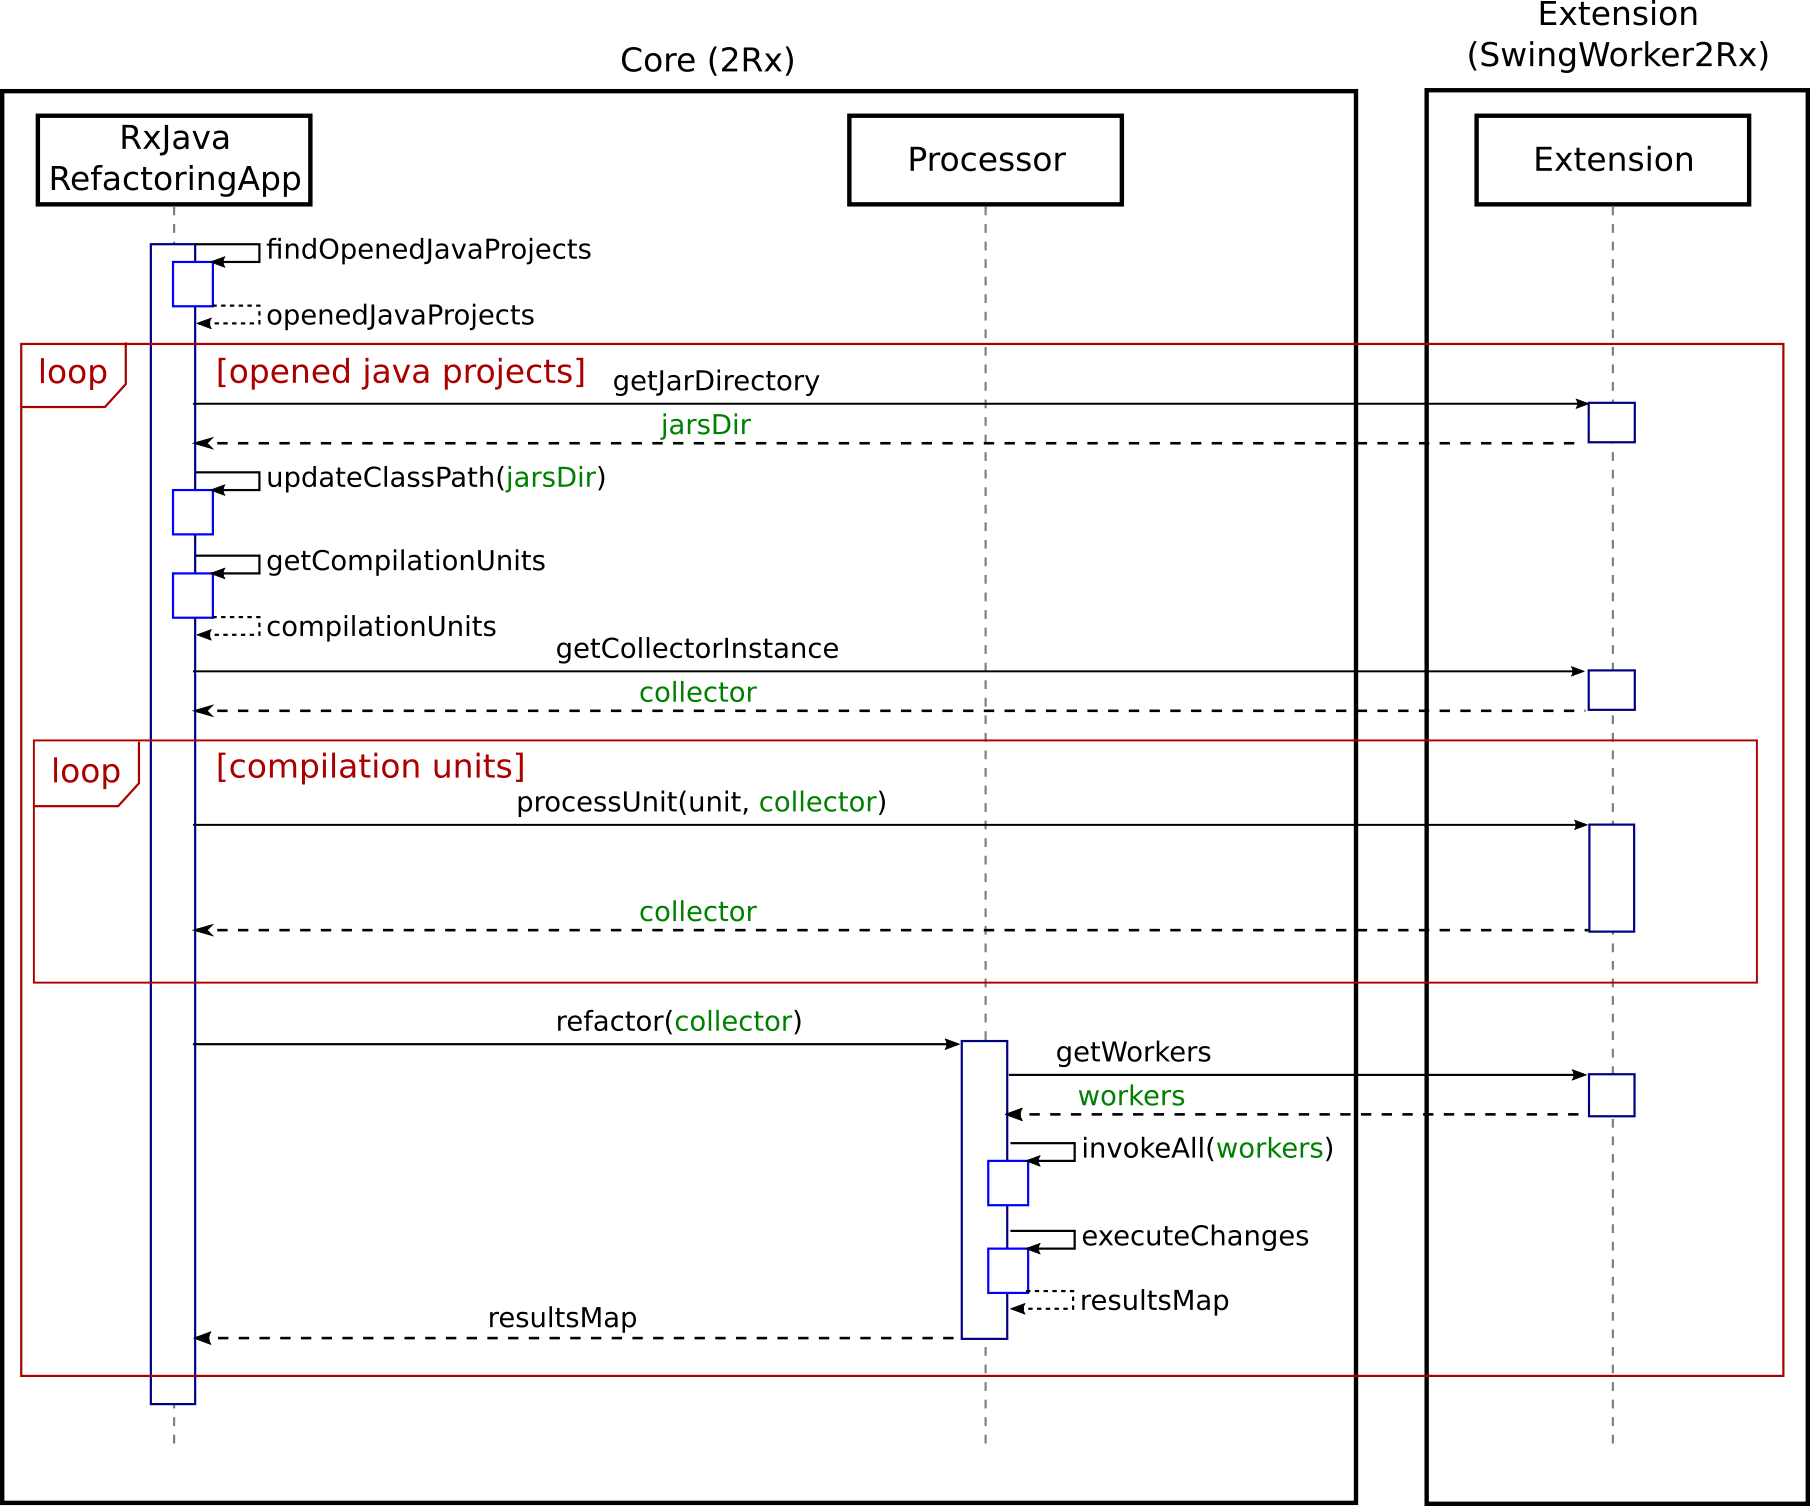
\includegraphics[width=15cm]{design/plugin-design.png}
\end{center}
\caption{Plugin Design}
\label{fig:plugin-design}
\end{figure}

\begin{figure}[H]
\begin{center}
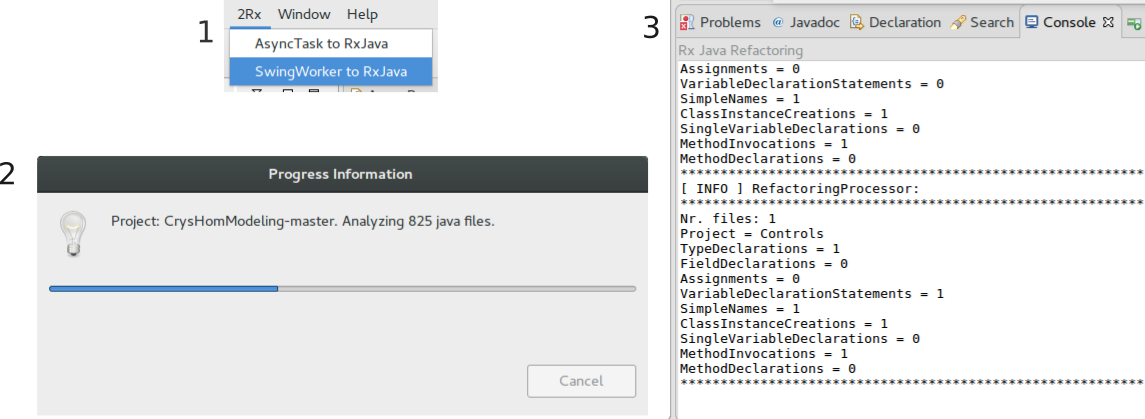
\includegraphics[width=15cm]{design/tool-ui.png}
\end{center}
\caption{\toolcore{} and \toolextension{}}
\label{fig:tool-ui}
\end{figure}

\toolcore{} also provides its clients with utility classes and a code generator. The utility classes offer a variety of methods to query information about AST nodes, perform code transformations directly in the AST, send log messages to the console, validate source code strings, among others. The code generator corresponds to a class that contains methods to create several AST node types from source code. The supported AST nodes are single statements, blocks of statements, method declarations, type declarations and field declarations. Defining these AST nodes with JDT (Eclipse Java Development Tools) in the conventional way usually requires a lot of code because every node of the target syntax tree must be specified. Generating these AST nodes from text facilitates the implementation and maintenance.

\subsection{Extension Setup}
\toolcore{} provides an extension point that allows adding clients to the plugin without modifying the existing code. In this extension point we specified that clients must implement the interface \code{RxJavaRefactoringExtension} (Listing~\ref{code:extension-interface}).

\begin{figure}[H]
\begin{sourcecode}
\begin{javacode}{}
public interface RxJavaRefactoringExtension<CollectorType extends AbstractCollector> {
	CollectorType getASTNodesCollectorInstance(IProject project);
	void processUnit( ICompilationUnit unit, CollectorType collector );
	Set<AbstractRefactorWorker<CollectorType>> getRefactoringWorkers( CollectorType collector );
	String getId();
	default String getJarFilesPath() { return null;}
}
\end{javacode}
\caption{Extension Interface}
\label{code:extension-interface}
\end{sourcecode}
\end{figure}

Additionally, we created a template project facilitate the implementation of extensions. This project contains a \code{README} file that explains how to setup the template. The template contains a default package structure. The action handler in the extension is already implemented. This handler is in charge of forwarding the action event to \toolcore{}. \toolcore{} reads the command id from the event to identify which extension triggered operation. There is also a default implementation of the \code{RxJavaRefactoringExtension} interface. This file contains placeholders in string values that must be replaced and TODOs in methods that must be implemented.

\subsection{Test-Driven Development}
We also developed a third project for test-driven development. This project only contains tests. The main idea is to have a basic project containing the cases to be tested. Each file contains a single case (Figure~\ref{fig:unit-test-results}). Additionally, there is a second folder containing all expected \framework{Java} classes, which are used for the assertions.

When the tests are executed, the basic project is refactored without writing the changes to the files. In this way, we guarantee that the input files never change and can always be reused. The resulting code of each compilation unit is saved in a map. For the comparison, we generate an AST for output and expected file. Then the trees are compared. The purpose of doing this is to ignore irrelevant differences such as spaces, empty lines, comments, etc.

Similar to the extensions, there is a template to facilitate setting up the project for the unit tests. This template contains abstract tests classes that can be used to load \framework{Android} or \framework{Java} projects, create \framework{Java} projects and assert source code based on string values.

\begin{figure}[H]
\begin{center}
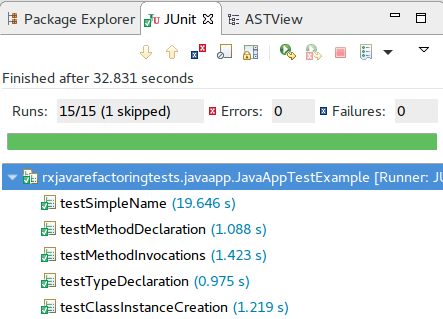
\includegraphics[height=5cm]{unit-tests/unit-tests-results1.png}
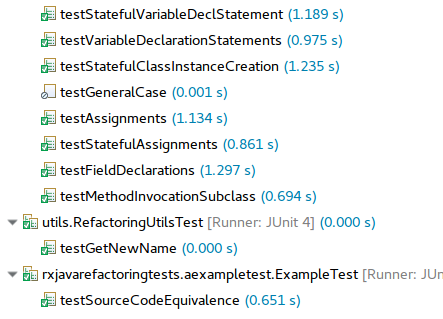
\includegraphics[height=5cm]{unit-tests/unit-tests-results2.png}
\end{center}
\caption{Unit Test Results}
\label{fig:unit-test-results}
\end{figure}

\chapter{Implementation of the System}
\label{chapter:implementation}
The refactoring approach used by \toolextension{} is based on the implementation of three classes that complement \framework{RxJava}. In this chapter, we explain how these classes work. Furthermore, we present some refactoring examples for different AST nodes (input vs. output). After that, we focus on the implementation of \toolextension{} and finally we talk about the template projects available that can be used to implement and test extensions.

\section{RxJava Extension}

We developed an extension to support the \code{SwingWorker} API in \framework{RxJava}. This extension consist of an \code{Emitter}, a \code{Package} and a \code{Subscriber} class. To identify these classes we added the prefix \code{SW} to their names. 

\begin{figure}[h]
\begin{center}
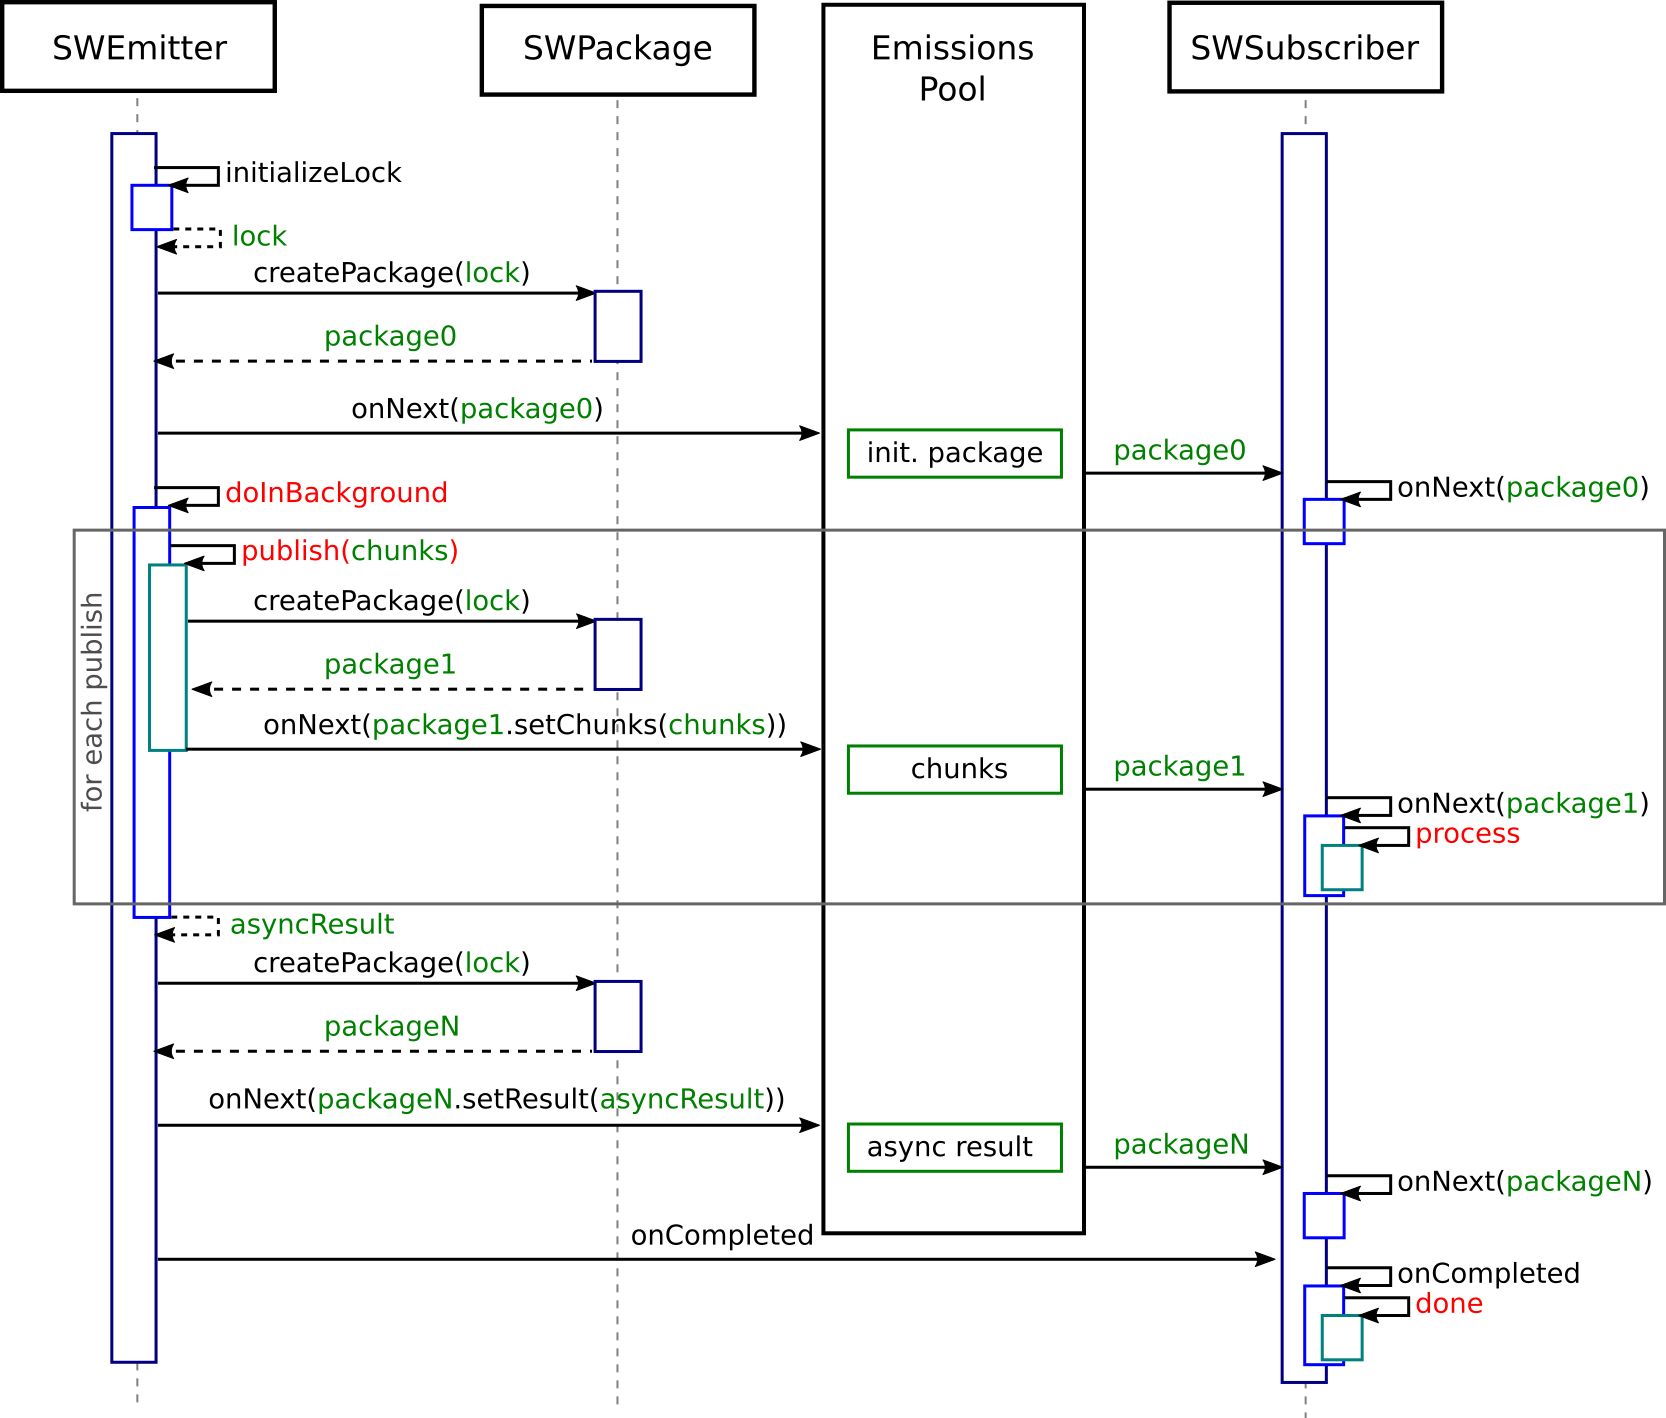
\includegraphics[width=17cm]{design/rxjava-extension.png}
\end{center}
\caption{RxJava Extension for SwingWorkers}
\label{fig:rxjava-extension}
\end{figure}

Figure~\ref{fig:rxjava-extension} shows the interactions between these three classes. In general, the \code{SWEmitter} produces \code{SWPackage}s that go into an ``Emissions Pool'', then the \code{SWSubscriber} takes those packages and process them. The \code{SWPackage} has two functions. The first one is to manage synchronization to avoid backpressure problems. The second one is to encapsulate the data into a single data structure. This is necessary because \code{Subscriber}s in \framework{RxJava} only accept one type, but the \code{SWEmitter} produces \code{Integer}s for reporting progress, another type for intermediate results and it can use a different one for the final result. The method \code{doInBackground} from the \code{SWEmitter} is an abstract method, while the methods \code{process} and \code{done} from the \code{SWSubscriber} possess a default implementation that can be overridden by subclasses. The default implementation does not possess any logic, it only avoids forcing developers to declare this method in the subclass.

The process starts by initializing a \code{lock} in the \code{SWEmitter}. This \code{lock} is used for all \code{SWPackage}s. Then an initialization \code{SWPackage} is created and sent to the emissions pool. After that, the asynchronous operation starts (\code{doInBackground}). While this operation is running, the methods \code{publish} or \code{setProgress} can be invoked multiple times. This invocations also generate \code{SWPackage}s that are pushed into the emissions pool, where they are taken and processed from the \code{SWSubscriber}. If the emission was generated by a \code{publish} invocation then the \code{process} method of the \code{SWSubscriber} will be invoked. When the asynchronous operations finishes, a final \code{SWPackage} containing the result is sent to the emissions pool again. Finally, the \code{onCompleted} method of the \code{SWSubscriber} is invoked. This method triggers the piece of code contained in the \code{done} method of the \code{SWSubscriber}.

While the \code{SWPackage}s are being processed, the \code{SWSubscriber} updates the state of the operation (\code{PENDING}, \code{STARTED}, \code{DONE}). The \code{SWSubscriber} contains all methods available in the \code{SwingWorker} API including the state relevant ones.

\subsection{Package Data Structure}
\label{sec:imp-package}
The main purpose of the \code{SWPackage} is to manage synchronization and encapsulate different types of data. Listings~\ref{code:swpackage-contain} how these fields are defined in the generic class. The progress is defined as an \code{AtomicInteger} to make the variable thread-safe. The other two types can only be accessed through getters and setters that use locks to guarantee thread-safe access. The \code{processingLock} is shared among all \code{SWPackage}s. This object comes from the \code{SWEmitter} and is the one that allows us to avoid backpressure problems.

\begin{figure}[h]
\begin{sourcecode}
\begin{javacode}{}
public final class SWPackage<ReturnType, ProcessType> {
	...
	private ReturnType asyncResult;
	private List<ProcessType> chunks;
	private AtomicInteger progress;
	private ReentrantLock processingLock;
	private Object asyncResultLock;

	SWPackage(ReentrantLock processingLock ) {
		this.processingLock = processingLock;
		...
	}
	...
}
\end{javacode}
\caption{SWPackage Contents}
\label{code:swpackage-contain}
\end{sourcecode}
\end{figure}

\subsection{Emitter}
\label{sec:imp-emitter}
The \code{SWEmitter} generates the packages that are going to be processed by the \code{SWSubscriber}. Listings~\ref{code:swemitter-regular-emissions} shows the implementation of the standard emissions in a \code{SWEmitter}. We call them standards because they are always produced. There are two emissions of this kind, initialization and result. Notice that \code{setResult} returns an \code{SWPackage} as well, otherwise, it would not be possible to use this call as a parameter for \code{onNext}.

\begin{figure}[h]
\begin{sourcecode}
\begin{javacode}{}
...
	this.emitter.onNext( createPackage() ); // init
	ReturnType asyncResult = doInBackground();
	this.emitter.onNext( createPackage().setResult( asyncResult ) ); // result
...
\end{javacode}
\caption{SWEmitter Standard Emissions}
\label{code:swemitter-regular-emissions}
\end{sourcecode}
\end{figure}

The \code{doInBackground} method is abstract and must therefore be implemented in the subclass. This implementation can invoke the \code{publish} and/or the \code{setProgress} method multiple times. If these methods are invoked, then they are forward to the \code{SWSubscriber} using a \code{SWPackage} as well. Listings~\ref{code:swemitter-dynamic-emissions} shows how the forwarding was implemented. Notice that \code{setChunks} and \code{setProgress} return an \code{SWPackage} as well.

\begin{figure}[H]
\begin{sourcecode}
\begin{javacode}{}
public abstract class SWEmitter<ReturnType, ProcessType> 
	implements Action1<Emitter<SWPackage<ReturnType, ProcessType>>>
	...
	@Override
	public final void call( Emitter<SWPackage<ReturnType, ProcessType>> emitter ) {
		... 
		// Template Method Pattern:
		// The doInBackground method (implemented in the subclass) is invoked here
	}
	
	protected void publish( ProcessType... chunks ) {
		this.emitter.onNext( createPackage().setChunks( chunks ) );
	}
	...
	protected void setProgress( int progress ) {
		this.emitter.onNext( createPackage().setProgress( progress ) );
	}
	...
\end{javacode}
\caption{SWEmitter Dynamic Emissions}
\label{code:swemitter-dynamic-emissions}
\end{sourcecode}
\end{figure}

\subsection{Subscriber}
\label{sec:imp-subscriber}
The \code{SWSubscriber} is the class responsible for managing state related operations that were present in the \code{SwingWorker}. In order to manage stateful operations, it is necessary to have private fields that can be updated on specific events. Listings~\ref{code:swsubscriber-state-relevant-fields} shows the fields required to implement all methods available in the \code{SwingWorker} API. These fields allow the implementation of the following methods:

\begin{itemize}
	\item \code{propertyChangeSupport}: \java{addPropertyChangeListener}, \java{firePropertyChange}, \java{getPropertyChangeSupport} and \java{removeProperyChangeListener}
	\item \code{progress}: \java{setProgress} and \java{getProgress}
	\item \code{cancelled}: \java{isCancelled}
	\item \code{currentState}: \java{getState} and \java{isDone}
\end{itemize}

\begin{figure}[h]
\begin{sourcecode}
\begin{javacode}{}
...
	private PropertyChangeSupport propertyChangeSupport;
	private AtomicInteger progress;
	private AtomicBoolean canceled;
	private SwingWorker.StateValue currentState;
...
\end{javacode}
\caption{State relevant Fields in SWSubscribers}
\label{code:swsubscriber-state-relevant-fields}
\end{sourcecode}
\end{figure}

At the beginning, the state of the \code{SWSubscriber} is \code{PENDING}. When the operation starts, the method \code{onStart} from the \code{SWSubscriber} is invoked, making the status change to \code{STARTED} (Listing~\ref{code:swsubscriber-onstart}). We use the \code{countDownLatch} to be able to wait for the asynchronous result when the \code{get} method is invoked. This is necessary because the \code{SwingWorker} API specifies that \code{get} is blocking.

\begin{figure}[h]
\begin{sourcecode}
\begin{javacode}{}
public final void onStart() {
	initialize(); // progress = 0; cancelled = false;
	this.countDownLatch = new CountDownLatch( 1 );
	setState( SwingWorker.StateValue.STARTED );
}
\end{javacode}
\caption{SWSubscriber onStart}
\label{code:swsubscriber-onstart}
\end{sourcecode}
\end{figure}

Listing~\ref{code:swsubscriber-onnext} shows how the \code{SWSubscriber} processes the \code{SWPackage}. First, it updates the async result. If no result is present, then the value remains \code{null}. Then it checks whether a progress value was sent and if so, it updates the \code{progress} field. Finally, if the \code{publish} method in the \code{SWEmitter} was invoked, the data is taken and processed in the \code{process} method.

Listings~\ref{code:swsubscriber-oncompleted} shows the termination of emissions. At the end, the \code{onCompleted} method of the \code{SWSubscriber} is invoked. Here the \code{countDownLatch} is decrease by one to report that the asynchronous operation has finished. Then the \code{done} method of the \code{SWSubscriber} is invoked and finally the state is set to \code{DONE}.

\begin{figure}[H]
\begin{minipage}{0.61\textwidth}
\begin{sourcecode}
\begin{javacode}{}
public final void onNext(SWPackage<ResultType,ProcessType> swPackage){
	...
	asyncResult = swPackage.getResult();
	if ( swPackage.isProgressValueAvailable() )
		setProgress(swPackage.getProgressAndReset());

	if ( !swPackage.getChunks().isEmpty() )
		process(swPackage.getChunks());
}
\end{javacode}
\caption{SWSubscriber onNext}
\label{code:swsubscriber-onnext}
\end{sourcecode}
\end{minipage}\hspace{0.65cm}
\begin{minipage}{0.35\textwidth}
\begin{sourcecode}
\begin{javacode}{}
public final void onCompleted() { 
	countDownLatch.countDown();
	done();
	setState(SwingWorker.StateValue.DONE);
}
\end{javacode}
\caption{SWSubscriber onCompleted}
\label{code:swsubscriber-oncompleted}
\end{sourcecode}
\end{minipage}
\end{figure}

The \code{SWSubscriber} implements all methods available in the \code{SwingWorker} API. Explaining how they are implemented would require copying the source code of the whole class in this section. Therefore we have limited ourselves to explain the \framework{RxJava} related methods.


\section{Refactoring Approach}
In this thesis, we propose a refactoring approach that allows transforming \code{SwingWorker}s to \framework{RxJava} by modifying a few lines of the source code. This is possible because the \code{SwingWorker} workflow is imitated through the interaction between \code{SWEmitter}, \code{SWPackage} and \code{SWSubscriber}.

In the following subsections, we explain how we refactore different AST nodes. These code snippets can be compared to the example shown at the beginning of Chapter~\ref{chapter:design}, to understand how the transformations in the Juneiform application were performed (Listings~\ref{code:example-original},~\ref{code:example-refactored}).

On the left side we present the original source code and on the right side the refactored one.

\subsection{Assignments}
The usage of the AST node \code{Assignment} involves working with variables. We observed that often the variable names contain the substrings ``swingWorker'' or     ``worker''. Since we are refactoring this construct, we replace these substrings by ``rxObserver''.

\begin{figure}[H]
\begin{minipage}{0.48\textwidth}
\begin{sourcecode}
\begin{javacode}{}
anotherWorker = swingWorker;
\end{javacode}
\caption{Assignment before Refactoring}
\label{code:assigment-before}
\end{sourcecode}
\end{minipage}\hspace{0.7cm}
\begin{minipage}{0.48\textwidth}
\begin{sourcecode}
\begin{javacode}{}
anotherRxObserver = rxObserver;
\end{javacode}
\caption{Assignment after Refactoring}
\label{code:assigment-after}
\end{sourcecode}
\end{minipage}
\end{figure}

There are also cases where a variable can be directly assigned to a class instance creation. The refactoring of class instance creations is shown in subsection~\ref{sec:imp-class-instance-creations}.

\subsection{Variable Declaration Statements}
Similar to \code{Assignment}s, \code{SingleVariableDeclaration}s involve variable names that must be adjusted. Additionally, the data type \code{SwingWorker} must be changed to \code{SWSubscriber} (Listings~\ref{code:vds-before} and ~\ref{code:vds-after}).

\begin{figure}[H]
\begin{minipage}{0.48\textwidth}
\begin{sourcecode}
\begin{javacode}{}
SwingWorker anotherWorker = swingWorker;
\end{javacode}
\caption{Variable Declaration Statement\\before Refactoring}
\label{code:vds-before}
\end{sourcecode}
\end{minipage}\hspace{0.7cm}
\begin{minipage}{0.48\textwidth}
\begin{sourcecode}
\begin{javacode}{}
SWSubscriber anotherRxObserver = rxObserver;
\end{javacode}
\caption{Variable Declaration Statement\\after Refactoring}
\label{code:vds-after}
\end{sourcecode}
\end{minipage}
\end{figure}

It is also possible to have \code{ClassInstanceCreation}s in \code{VariableDeclarationStatements} AST nodes. See subsection~\ref{sec:imp-class-instance-creations} for more details about the refactoring of \code{ClassInstanceCretion} nodes.

\subsection{Class Instance Creations}
\label{sec:imp-class-instance-creations}
\code{ClassInstanceCreation}s are the AST nodes that actually contain the implementation of the \code{SwingWorker}. During the refactoring, we separate this implementation into two objects. The \code{Observable} and the \code{SWSubscriber}. The \code{Observable} contains the logic for the asynchronous operation, while the \code{SWSubscriber} has the logic responsible for processing both types of results, intermediate and final. The \code{SWEmitter} and the \code{SWSubscriber} were designed to support the protected methods of the \code{SwingWorker} API. Therefore the blocks \code{doInBackground}, \code{process} and \code{done} do not need to be modified (Listings~\ref{code:cic-before} and~\ref{code:cic-after}).

\begin{figure}[H]
\begin{minipage}{0.48\textwidth}
\begin{sourcecode}
\begin{javacode}{1-2}
SwingWorker<String, Integer> swingWorker 
	= new SwingWorker<String, Integer>() {
	@Override
	protected String doInBackground() throws Exception {
		...
	}
	protected void process(List<Integer> chunks){...}
	protected void done() {...}
};
\end{javacode}
\caption{Class Instance Creation before Refactoring}
\label{code:cic-before}
\end{sourcecode}
\end{minipage}\hspace{0.7cm}
\begin{minipage}{0.48\textwidth}
\begin{sourcecode}
\begin{javacode}{1-3,9,11-12}
rx.Observable<SWPackage<String, Integer>> rxObservable 
	= rx.Observable
		.fromEmitter(new SWEmitter<String, Integer>() {
			@Override
			protected String doInBackground() 
			throws Exception {
				...
			}
}, Emitter.BackpressureMode.BUFFER );

SWSubscriber<String, Integer> rxObserver 
	= new SWSubscriber<String, Integer>(rxObservable) {
	protected void process(List<Integer> chunks){...}
	protected void done() {...}
};
\end{javacode}
\caption{Class Instance Creation after Refactoring}
\label{code:cic-after}
\end{sourcecode}
\end{minipage}
\end{figure}


\subsection{Field Declarations}
\code{FieldDeclaration}s are very similar to \code{VariableDeclarationStatement}s. Normally, it is only necessary to adjust the variable name and change the data type from \code{SwingWorker} to \code{SWSubscriber}. However, we do have an important special case for \code{FieldDeclaration}s. Our approach creates two objects out of a \code{SwingWorker} and the constructor of the \code{SWSubscriber} requires an \code{Observable}. To make the code more readable, we decided to create an inner class that extends \code{SWSubscriber} and generate the \code{Observable} there (Listings~\ref{code:fd-before} and~\ref{code:fd-after}).

\begin{figure}[H]
\begin{minipage}{0.48\textwidth}
\begin{sourcecode}
\begin{javacode}{1,2}
private SwingWorker<String, Integer> anotherWorker 
	= new SwingWorker<String, Integer>(){
	@Override
	protected String doInBackground() throws Exception
	{
		...
	}
	protected void process( List<Integer> chunks ) {...}
	protected void done() {...}
};
\end{javacode}
\caption{Field Declaration before Refactoring}
\label{code:fd-before}
\end{sourcecode}
\end{minipage}\hspace{0.7cm}
\begin{minipage}{0.48\textwidth}
\begin{sourcecode}
\begin{javacode}{1,2,4,5,7-10,16}
private SWSubscriber<String,Integer> anotherRxObserver 
	= new RxObserver();

class RxObserver extends SWSubscriber<String,Integer>{
	RxObserver(){ setObservable(getRxObservable()); }

	private rx.Observable<SWPackage<String, Integer>> 
		getRxObservable() {
		return rx.Observable.fromEmitter( 
			new SWEmitter<String, Integer>() {
				@Override
				protected String doInBackground() 
				throws Exception {
					...
				}
		}, Emitter.BackpressureMode.BUFFER );
	}
	protected void process( List<Integer> chunks ) {...}
	protected void done() {...}
}
\end{javacode}
\caption{Field Declaration after Refactoring}
\label{code:fd-after}
\end{sourcecode}
\end{minipage}
\end{figure}

Another alternative for refactoring this kind of \code{FieldDeclaration}s is to write the \code{Observable} directly in the constructor (See Listing~\ref{code:fd-alternative}), but in our opinion, this code is harder to read, specially if the method \code{doInBackground} has many lines.

\begin{figure}[H]
\begin{sourcecode}
\begin{javacode}{2-7}
private SWSubscriber<String, Integer> anotherRxObserver = new SWSubscriber<String, Integer>(
			rx.Observable.fromEmitter( 
				new SWEmitter<String, Integer>() {
					@Override
					protected String doInBackground() 
					throws Exception {...}
			}, Emitter.BackpressureMode.BUFFER )
	) {
	protected void process( List<Integer> chunks ) {...}
	protected void done() {...}
};	
\end{javacode}
\caption{Alternative Refactoring for Field Declaration}
\label{code:fd-alternative}
\end{sourcecode}
\end{figure}

\code{SwingWorker}s can also contain custom fields and/or methods. In these cases, we also use an inner class such as \code{RxObserver}, shown in Listing~\ref{code:fd-after}, that contains all of the custom fields and methods. By doing that we guarantee, that the pieces of code contained in the \code{Observable} and the \code{SWSubscriber} still have access to those elements.

\subsection{Method Declaration}
We also modify \code{MethodDeclaration}s to adjust the return value from \code{SwingWorker} to \code{SWSubscriber} (Listings~\ref{code:md-before} and~\ref{code:md-after}).

\begin{figure}[H]
\begin{minipage}{0.48\textwidth}
\begin{sourcecode}
\begin{javacode}{1}
private SwingWorker<String, Integer> 
	getSwingWorker(){ ... }
\end{javacode}
\caption{Method Declaration before Refactoring}
\label{code:md-before}
\end{sourcecode}
\end{minipage}\hspace{0.7cm}
\begin{minipage}{0.48\textwidth}
\begin{sourcecode}
\begin{javacode}{1}
private SWSubscriber<String, Integer> 
	getSwingWorker(){ ... }
\end{javacode}
\caption{Method Declaration after Refactoring}
\label{code:md-after}
\end{sourcecode}
\end{minipage}
\end{figure}

\subsection{Method Invocations}
Only three methods out of eighteen were renamed in the \code{SWSubscriber}. The refactoring of \code{MethodInvocation} nodes also involves checking the name of the invokers and adjusting them if necessary. The substrings ``swingWorker'' and ``worker'' are replaced by ``rxObserver''. Listings~\ref{code:mi-before} and~\ref{code:mi-after} shows the refactoring of the only methods that were renamed.

\begin{figure}[H]
\begin{minipage}{0.48\textwidth}
\begin{sourcecode}
\begin{javacode}{}
swingWorker.cancel( true );
swingWorker.execute();
swingWorker.run();
\end{javacode}
\caption{Method Invocations before Refactoring}
\label{code:mi-before}
\end{sourcecode}
\end{minipage}\hspace{0.7cm}
\begin{minipage}{0.48\textwidth}
\begin{sourcecode}
\begin{javacode}{}
rxObserver.cancelObservable( true );
rxObserver.executeObservable();
rxObserver.runObservable();
\end{javacode}
\caption{Method Invocations after Refactoring}
\label{code:mi-after}
\end{sourcecode}
\end{minipage}
\end{figure}

\subsection{Simple Names}
We refactor \code{SimpleName}s to adjust the argument name of \code{SwingWorker} types in invocations (Listings~\ref{code:sn-before} and~\ref{code:sn-after}).

\begin{figure}[H]
\begin{minipage}{0.48\textwidth}
\begin{sourcecode}
\begin{javacode}{}
doSomething( swingWorker );
\end{javacode}
\caption{Simple Name before Refactoring}
\label{code:sn-before}
\end{sourcecode}
\end{minipage}\hspace{0.7cm}
\begin{minipage}{0.48\textwidth}
\begin{sourcecode}
\begin{javacode}{}
doSomething( rxObserver );
\end{javacode}
\caption{Simple Name after Refactoring}
\label{code:sn-after}
\end{sourcecode}
\end{minipage}
\end{figure}

\subsection{Single Variable Declarations}
\code{SwingWorker}s can also be parameters of methods. The variables defined in a \code{MethodDeclaration} are called \code{SingleVariableDeclaration}. We use this AST node to refactor refactor these \code{SwingWorker}s into \code{SWSubscriber}s (Listings~\ref{code:svd-before} and~\ref{code:svd-after}).

\begin{figure}[H]
\begin{minipage}{0.48\textwidth}
\begin{sourcecode}
\begin{javacode}{}
void doSomething ( SwingWorker swingWorker ) {...}
\end{javacode}
\caption{Single Variable Declaration before Refactoring}
\label{code:svd-before}
\end{sourcecode}
\end{minipage}\hspace{0.7cm}
\begin{minipage}{0.48\textwidth}
\begin{sourcecode}
\begin{javacode}{}
void doSomething ( SWSubscriber rxObserver ) {...}
\end{javacode}
\caption{Single Variable Declaration after Refactoring}
\label{code:svd-after}
\end{sourcecode}
\end{minipage}
\end{figure}

\subsection{Type Declarations}
In order to refactor \code{TypeDeclaration} nodes, it is necessary to change the superclass of the target node from \code{SwingWorker} to \code{SWSubscriber}. Furthermore, we need to set the \code{Observable} in the constructor. Listings~\ref{code:td-before} and~\ref{code:td-after} illustrate how this is done. Notice that the method \code{getRxObservable} is the same that we use for the special case of \code{FieldDeclaration}s (Listing~\ref{code:fd-after}).

\begin{figure}[H]
\begin{minipage}{0.48\textwidth}
\begin{sourcecode}
\begin{javacode}{2}
public class ClassA 
	extends SwingWorker<String, Integer> {
	...
	public ClassA(...) {
		...	
	}
}
\end{javacode}
\caption{Type Declaration before Refactoring}
\label{code:td-before}
\end{sourcecode}
\end{minipage}\hspace{0.7cm}
\begin{minipage}{0.48\textwidth}
\begin{sourcecode}
\begin{javacode}{2,6,9-12}
public class ClassA 
	extends SWSubscriber<String, Integer> {
	...
	public ClassA(...) {
		...
		setObservable( getRxObservable() );
	}
	
	private rx.Observable<SWPackage<String, Integer>> 
		getRxObservable() {
			return rx.Observable.fromEmitter( ... );
	}
}
\end{javacode}
\caption{Type Declaration after Refactoring}
\label{code:td-after}
\end{sourcecode}
\end{minipage}
\end{figure}

\section{\toolcore{} and \toolextension{}}
\toolcore{} and \toolextension{} work together to perform the automated refactoring of \code{SwingWorker}s to \code{RxJava}. The first step to implement an extension of \toolcore{} is to define its id, name and the location of its resources (i.e. required jar files). After that, the object responsible for collecting all relevant AST nodes for the refactoring must be implemented. To refactor \code{SwingWorker}s it is necessary to collect the following AST nodes: \code{TypeDeclaration}, \code{FieldDeclarations}, \code{Assignment}, \code{VariableDeclarationStatement}, \code{SimpleName}, \code{ClassIntanceCreation}, \code{SingleVariableDeclaration}, \code{MethodInvocation} and \code{MethodDeclaration}.


\subsection{Collectors}
The collector has a \code{Map} for each of these fields. The \code{Map} holds compilation units and a list of the corresponding node. Listing~\ref{code:collector} shows an example of the fields that we use for the collector of \toolextension{}.

\begin{figure}[H]
\begin{sourcecode}
\begin{javacode}{}
public class RxCollector extends AbstractCollector {
	...
	private final Map<ICompilationUnit, List<TypeDeclaration>> typeDeclMap;
	private final Map<ICompilationUnit, List<FieldDeclaration>> fieldDeclMap;
	// etc...
}
\end{javacode}
\caption{\toolextension{} Collector}
\label{code:collector}
\end{sourcecode}
\end{figure}

\subsection{Processing}
At the beginning the collector is empty. The collector is updated on each \code{processUnit} invocation (Figure~\ref{fig:plugin-design}). Since the collector only holds the nodes, another object is needed to analyze the current unit. For that purpose, we use a class that extends \code{ASTVisitor}. The visitor iterates through all nodes of the compilation units and adds the relevant nodes to a list containing the corresponding node type. There are as many \code{List}s in the visitor as \code{Map}s in the collector.

The difference between the visitor and the collector is that a new visitor instance is used for each compilation unit, meaning that a visitor only contains the relevant information for a single compilation unit, while the collector contains all the relevant nodes for the whole project. Listing~\ref{code:processing} shows how the visitor and the collector interact with each other.

\begin{figure}[H]
\begin{sourcecode}
\begin{javacode}{12-14}
@Override
public void processUnit( ICompilationUnit unit, RxCollector rxCollector ) {
	...
	// Initialize Visitor
	String className = SwingWorkerInfo.getBinaryName();
	DiscoveringVisitor discoveringVisitor = new DiscoveringVisitor( className );

	// Collect information using visitors
	compilationUnit.accept( discoveringVisitor );

	// Cache the collected information from visitors in one collector
	rxCollector.add( unit, discoveringVisitor.getTypeDeclarations() );
	rxCollector.add( unit, discoveringVisitor.getFieldDeclarations() );
	rxCollector.add( unit, discoveringVisitor.getAssignments() );
	// etc...
}
\end{javacode}
\caption{\toolextension{} Processing Compilation Units}
\label{code:processing}
\end{sourcecode}
\end{figure}


\subsection{Workers}
When all compilation units have been processed, then \toolcore{} uses the collector and a set of workers provided by the extension (See Figure~\ref{fig:plugin-design}) to perform the refactorings. In order to have workers with clear responsibilities and avoid long classes, we implemented a worker for each \code{ASTNode} present in the collector. That makes a total of nine workers.

Listing~\ref{code:workers-pseudo-code} presents the refactoring algorithm used. First, we get the corresponding map from the collector. For each entry in this map, we take the key, which corresponds to a compilation unit. Then, we iterate trough the values of each map entry. The values correspond to the target nodes. In each of these nodes, we run a refactoring visitor that performs a static analysis and caches all relevant information. Then we apply the refactorings using the abstract syntax tree, the compilation unit, the visitor, the single unit writer and the target node. Finally, we register the current compilation unit into the multiple units writer.

The single unit writer does not modify either the compilation units nor the abstract syntax trees. Instead, it registers the changes in a \code{ASTRewrite} object. By doing this we guarantee, that all workers have access to the original code. After all workers have been executed, the multiple units writer applies the changes to the compilation units.

\begin{figure}[H]
\begin{sourcecode}
\begin{javacode}{}
map = collector.xyzMap // assignmentMap, classInstanceCreationMap, etc...

for each map.entry entry
	compilationUnit = entry.key
	
	for each entry.values node
		ast = node.ast
		singleUnitWriter = WriterHolder.getSingleUnitWriterInstance( ast, compilationUnit )
		refactoringVisitor = new RefactoringVisitor
		node.accept( refactoringVisitor )		
		refactor( ast, compilationUnit, refactoringVisitor, singleUnitWriter, node )
		multipleUnitsWriter.addCompilationUnit( icu )
	
\end{javacode}
\caption{Worker's Pseudo Code}
\label{code:workers-pseudo-code}
\end{sourcecode}
\end{figure}

After we have implemented all workers, we add them to a set, which is used by \toolcore{} to refactor the original code. Listing~\ref{code:workers} shows how we build the set of workers.

\begin{figure}[H]
\begin{sourcecode}
\begin{javacode}{}
@Override
public Set<AbstractRefactorWorker<RxCollector>> getRefactoringWorkers( RxCollector rxCollector ) {
	...
	Set<AbstractRefactorWorker<RxCollector>> workers = new HashSet<>();
	workers.add( new AssignmentWorker( rxCollector ) );
	workers.add( new FieldDeclarationWorker( rxCollector ) );
	workers.add( new MethodInvocationWorker( rxCollector ) );
	// etc...
}
\end{javacode}
\caption{\toolextension{} Providing Workers}
\label{code:workers}
\end{sourcecode}
\end{figure}

\subsection{Writers}
It is possible to extend the \code{RxSingleUnitWriter}, explained in Section~\ref{sec:core-components}, to support transformations that might not have been considered in \toolcore{}. Since all workers are executed simultaneously it is important to make sure that the methods here implemented are thread-safe. To accomplish that, we use the construct \code{synchronized}. Listing~\ref{code:rxsingleunitwriter-threadsafe} shows an example for replacing a \code{SimpleType}.

\begin{figure}[H]
\begin{sourcecode}
\begin{javacode}{}
@Override
public synchronized void replaceType( SimpleType oldType, String newType ) {
	AST ast = astRewriter.getAST();
	SimpleType newSimpleType = ast.newSimpleType( ast.newName( newType ) );
	astRewriter.replace( oldType, newSimpleType, null );
}
\end{javacode}
\caption{\toolcore{} RxSingleUnitWriter - Replace Type (Thread Safe)}
\label{code:rxsingleunitwriter-threadsafe}
\end{sourcecode}
\end{figure}

\subsection{Source Code Generation}
\toolcore{} provides a couple of methods that can be used to generate code from a string (source code). By using these methods and \framework{FreeMarker}~\cite{freeMarker} templates, we generate source code without having to specify all nodes using JDT. Listing~\ref{code:subscriber-ftl} shows the template used for generating inner class \code{RxSubscriber} shown in Listing~\ref{code:cic-after}. Basically, there is a \framework{Java} object called \code{model} that contains all necessary information for filling up the templates. This object is passed to the \framework{FreeMarker} processor in order to produce the source code.

\begin{figure}[H]
\begin{sourcecode}
\begin{javacode}{}
class ${model.className} extends SWSubscriber<${model.resultType}, ${model.processType}>{

<#list model.fieldDeclarations as fieldDeclaration> ${fieldDeclaration} </#list>

${model.className}() { setObservable(getRxObservable()); }

<#include "getRxObservable.ftl">
<#include "common/processBlock.ftl">
<#include "common/doneBlock.ftl">

<#list model.methods as method> ${method} </#list>

<#list model.typeDeclarations as typeDeclaration> ${typeDeclaration} </#list>
}
\end{javacode}
\caption{Subscriber Freemarker Template}
\label{code:subscriber-ftl}
\end{sourcecode}
\end{figure}

\section{Templates}
We developed two templates, to facilitate developing and testing extensions for \toolcore{}.

Figure~\ref{fig:template-ext} shows the package structure of the template design for extensions. The template consists of five classes. The \code{Handler} is already implemented. Its function is to forward the event to \toolcore{}. The classes \code{Extension}, \code{ExtCollector} and \code{FirstWorker} contains ``TODOs'' to facilitate their implementation. The name ``FirstWorker'' is a placeholder and should be renamed by developers to improve comprehension. The \code{SwingleUnitWriter} from \toolcore{} can directly be used by extensions. However, since the probability of having to add a method to this class is high, we added the \code{SingleUnitExtensionWriter} to the template, where new methods for manipulating the source code can be added.

Similarly, Figure~\ref{fig:template-test} shows the package structure of the template design for writing unit tests. This template consists of four abstract classes and three example tests classes. In order to be able to test \toolcore{} and its extensions, it is necessary to have an Eclipse project. These abstract classes open or create a project containing the input files. By using this templates developers can skip those steps and start writing the assertions they need. In Listing~\ref{code:unit-test-example} we show how a test would look like. The method \code{executeTest} is already implemented in the template project.

\begin{figure}[h]
\begin{subfigure}{0.5\textwidth}
\begin{center}
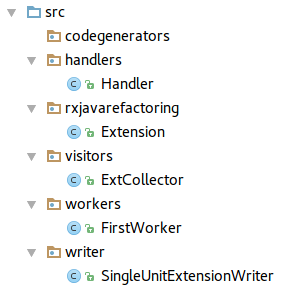
\includegraphics[width=5.5cm]{templates/extension.png}
\end{center}
\caption{Extension Template}
\label{fig:template-ext}
\end{subfigure}
\begin{subfigure}{0.5\textwidth}
\begin{center}
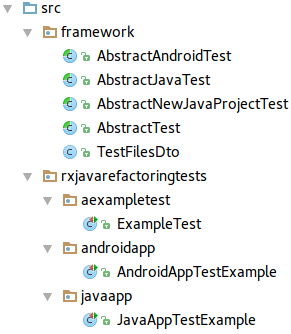
\includegraphics[width=5.5cm]{templates/tests.png}
\end{center}
\caption{Test Template}
\label{fig:template-test}
\end{subfigure}
\caption{Template Projects}
\end{figure}

\begin{figure}[H]
\begin{sourcecode}
\begin{javacode}{11-13,17}
public void testRefactoring() throws Exception {
	String targetFile = "FieldDeclaration.java";
	// getSourceCode( String ... path ) The name of the class does not need to match the name of the file
	String expectedSourceCode = getSourceCode( "expected.java.code", "FieldDeclarationRefactored.java" );
	executeTest( targetFile, expectedSourceCode );
}

private void executeTest( String targetFile, String expectedSourceCode ) throws Exception {
	RxJavaRefactoringApp app = new RxJavaRefactoringApp();
	Extension refactoringExtension = new Extension();
	app.setCommandId( refactoringExtension.getId() );
	app.setExtension( refactoringExtension );
	app.refactorOnly( targetFile );
	app.start( null );
	...
	String actualSourceCode = getSourceCodeByFileName( targetFile, results );
	assertEqualSourceCodes( expectedSourceCode, actualSourceCode );
}
\end{javacode}
\caption{Unit Test Example}
\label{code:unit-test-example}
\end{sourcecode}
\end{figure}

\chapter{Evaluation}
\label{chapter:evaluation}
We divided the evaluation into two parts. The first one corresponds to the accuracy of the refactoring approach, while the second one focuses on flexibility of the refactoring tool to support extensions.

\section{Refactoring Approach}
For the evaluation of the refactoring approach, we used 58 projects. One of these projects was developed for unit test. Ten projects were used for UI tests and the remaining 47 projects were used to analyze the original code versus the refactored code and check that there are no compilation errors.

\subsection{Dataset for Unit Tests}
We developed the project for unit tests the implementation phase following the test-driven development technique. Each unit tests is responsible for testing a specific refactoring worker. Therefore this project has at least one test file for each worker. The project contains also the refactored code, which is used to make sure that the output from \toolextension{} matches the expected file.

We did not only use this project for the implementation phase but also added to the final set of projects to be evaluated.

\subsection{Dataset for UI Tests}
We chose the projects for UI tests from Bitbucket according to the following criteria: small projects (less than 50 \framework{Java} files) that compile without having to setup a server, database, etc. We did not select these projects randomly because our goal was to be able to evaluate them at runtime and make sure that the behavior of the applications did not change. Randomly chosen applications are often not compilable due to missing files, complex setups, etc.

\subsection{Dataset for Source Code Analysis}
We used the remaining 47 projects to evaluate the refactoring tool by analyzing its output. We downloaded these projects randomly from Github. The search was performed using the Search site from Github ``\url{https://github.com/search}''. We used the following search parameters, Query: ``\code{SwingWorker}'', Language: \framework{Java}, Sort: Recently indexed. The equivalent search URL is: 
\begin{itemize}
	\item \url{https://github.com/search?l=Java&o=desc&q=SwingWorker&ref=searchresults&s=indexed&type=Code&utf8=\%E2\%9C\%93}
\end{itemize}

We did not consider further search parameters such as the number of stars or forks because the number of results was not representative. Table~\ref{table:results-starts-forks} shows an overview of the search results when using starts and/or forks as search parameters.

\begin{table}[h]
\begin{center}
\begin{tabular}{|p{5cm}|C{3cm}|}
\hline
\bf Criteria & \bf Nr. Results\\\hline
Stars $>$ 0 and Forks > 0 & 0\\
Stars $>$ 0 & 4\\
Forks $>$ 0 & 3\\
Stars $>$ 0 or Forks > 0 & 7\\
\hline
\end{tabular}
\end{center}
\caption{Search Results using Nr. of Starts and Forks}
\label{table:results-starts-forks}
\end{table}

From the result's list, we downloaded the first 50 Eclipse or Maven projects. Then we imported them into the Eclipse workspace to make sure that they compile. We analyzed projects that did not compile in order to determined whether the noncompilable source code was \code{SwingWorker} relevant or not. If the piece of code was not \code{SwingWorker} relevant, then we commented it out to hide the compilation errors shown in the IDE. Commenting out few lines of code does not affect the integrity of the evaluation because the projects were not meant to be tested at runtime. Three out of the fifty projects could not be properly setup to avoid compilation errors before refactoring. Therefore, we removed these projects from the final lists of projects to be evaluated.

\subsection{Results}
On the left side of Table~\ref{table:results} we show an overview of the results obtained after running \toolextension{} in the 58 projects. In total 14,930 lines of code were modified. This number includes the changes applied in the \code{.classpath} file, which are necessary to add the corresponding \code{.jar} files to the target project. From those 14,930 lines, two lines of code did not compile. These lines are explained in the next section. Appendix~\ref{appendix:eval-results-overview} shows the results of each project.

On the right side of Table~\ref{table:results} we show how many AST nodes containing \code{SwingWorker} were modified. \toolextension{} refactored 678 AST nodes in total. Appendix~\ref{appendix:eval-details} shows the results of each project.

\begin{table}[h]
\begin{center}
\begin{tabular}{|p{5cm}|C{2cm}|}
\hline
& \bf Total \\\hline
Projects & 58\\
Java Files & 10,055\\
Refactored Java Files & 180\\
Refactored Lines & 14,930\\
Lines with compile errors & 2\\
AST nodes & 678\\
Time & 5 min 17 s\\
\hline
\end{tabular}\hspace{1cm}
\begin{tabular}{|p{5cm}|C{2cm}|}
\hline
ASTNode & \bf Total\\\hline
TypeDeclaration & 78\\
FieldDeclaration & 42\\
Assignment & 41\\
VariableDeclarationStatement & 70\\
SimpleName & 116\\
ClassInstanceCreation & 146\\
SingleVariableDeclaration & 9\\
MethodInvocation & 171\\
MethodDeclaration & 5\\
\hline\hline
\bf Total & \bf 678\\
\hline
\end{tabular}
\end{center}
\caption{Refactoring Results}
\label{table:results}
\end{table}

The results presented above show that the refactoring approach presented in this thesis and the tool \toolextension{} are accurate. Only approximately 0.0001\% of the refactored lines showed compilation errors after refactoring. This lines, however, are not difficult to fix manually after the refactoring has completed.

\subsubsection{Limitations}
The current implementation of \toolextension{} makes impossible to refactor \code{SwingWorker} nodes found inside another \code{SwingWorker}. One of the two lines of code presenting compilation errors after refactoring corresponds to this case. 

Listing~\ref{code:nested-swingworkers} shows an example of this problem. Originally an \code{ExecutorService} submitted the instance \code{singleRun} by invoking \code{executorSC.submit(singleRun)}. Notice that \code{singleRun} is an instance of \code{SCWRLrunner}, which is a subclass of \code{SwingWorker}. This line was not refactored because the command is already within a \code{SwingWorker}. To fix this compilation error the line must be replaced by ``\java{singleRun.executeObservable()}''.

\begin{figure}[H]
\begin{sourcecode}
\begin{javacode}{7}
rx.Observable<SWChannel<Void, Void>> rxObservable = rx.Observable.fromEmitter(new SWEmitter<Void, Void>(){
	@Override
	protected Void doInBackground() throws Exception {
		...
					for (SCWRLrunner singleRun : SCWRLTasks) {
						...
						executorSC.submit(singleRun); // --> COMPILATION ERROR
					}
		...
	}
}, Emitter.BackpressureMode.BUFFER);
\end{javacode}
\caption{Project: CrysHomModeling-master\\ Class: modellingTool.MainMenu}
\label{code:nested-swingworkers}
\end{sourcecode}
\end{figure}


Another limitation found during the evaluation of the projects was conflicts between method names. Not all method names that can be used in \code{SwingWorker} subclasses, can also be used in \code{rx.Subscriber} subclasses. The second compilation error found corresponds to this case. 

Listing~\ref{code:method-name-conflict} shows an example of this problem. Since \code{SwingWorker}s do not have any method matching the name ``\code{add}'', the original code compiles. However the new subclass of \java{rx.Subscriber} does have an ``\code{add}'' method and therefore, the code does not compile. 

The solution is to replace line 6 by ``\java{AsyncPanel.this.add(targetComponent,}~\java{BorderLayout.CENTER);}'', since \code{AsyncPanel} is the name of the class containing the target method.

\begin{figure}[H]
\begin{sourcecode}
\begin{javacode}{6}
public AsyncPanel extends JPanel {
	private class InitWorker extends SWSubscriber<Void, Void> {
		...
	    protected void done() {
    	    ...
	        add(targetComponent, BorderLayout.CENTER); // --> COMPILE ERROR
        	...
    	}
	}
}
\end{javacode}
\caption{Project: trol-commander\\ Class: com.mucommander.ui.layout.AsyncPanel}
\label{code:method-name-conflict}
\end{sourcecode}
\end{figure}

\section{Generalization of the Tool}
In order to evaluate the flexibility of \toolcore{}, we refactored the implementation \textsc{RxFactor} to make it a client of \toolcore{}. This transformation did not require applying any modifications in \toolcore{}.

\subsection{Experimental Setup}
We took the same dataset used in \textsc{RxFactor} for the evaluation and compare the outputs of both tools, \textsc{RxFactor} and the extension of it for \toolcore{}.

\subsection{Validation Approach}
To validate that the extension of \textsc{RxFactor} and the original tool generate the same exact result, we refactored the \framework{Android} projects two times. The first time using \textsc{RxFactor} and the second time using the extension. We placed the output projects in different directories and ran the following Linux command to compare the directories, their files, and the contents of each file:

\begin{textcode}{}
diff -r rxfactor-original rxfactor-modified -x *.classpath -x *.project -x *.jar -x *.class
\end{textcode}

The argument \code{r} is used to specify that the command must be executed recursively (includes all subdirectories). The arguments \code{rxfactor-original} and \code{rxfactor-modified} correspond to the directories where we saved the outputs locally. Finally, we used the argument \code{x} to exclude the files with extensions \code{classpath}, \code{project}, \code{jar} and \code{class} in order to compare only \framework{Java} files.

\subsection{Results}
The ``diff'' command did not find any differences. That shows that the \textsc{RxFactor} was successfully adapted into an extension of \toolcore{}.

\chapter{Conclusion}
\label{chapter:conclusion}
Modern programming languages are making use of event-driven programming models and reactivity to facilitate both code writing and code comprehension, specially when developing asynchronous applications.

Asynchrony can improve the responsiveness of applications. Since refactoring asynchronous code is not trivial, researchers have developed tools to perform this task. Each tool targets a specific language and problem:

\begin{itemize}
	\item \textsc{PromisesLand} (JavaScript): converts asynchronous callbacks into \code{Promises}.
	\item \textsc{Asyncifer} (C\#): refactors callback-based asynchronous code into \code{async/wait} constructs
	\item \textsc{AsyncFixer} (C\#): finds anti-patterns of \code{async/wait} and suggest fixes
	\item \textsc{Asynchronizer} (Android): converts synchronous code into \code{AsyncTask}
	\item \textsc{AsyncDroid} (Android): converts \code{AsyncTask} into \code{IntentService}
	\item \textsc{RxFactor} (Android): converts \code{AsyncTask}s into \framework{RxJava}.
\end{itemize}

Previous studies have shown that these tools are needed, highly applicable and accurate~\cite{paperAsyncMobile, paperStudyRefactoring, thesisJavaScript}.

Furthermore, other studies agree that functional and reactive programming models improve code writing and code comprehension~\cite{promises, paperReactiveComprehension}. In this thesis, we show how to automatically refactor \code{SwingWorker}s into \framework{RxJava} in order to facilitate introducing reactive programming concepts in \framework{Java} applications that use this async construct. The results show that the developed tool is reliable. Only around $0.0001\%$ of the modified lines reported compile errors after the refactoring task has completed. One can, however, easily fix these errors manually.

\section{Future Work}

Since the plugin was divided into core (\toolcore{}) and extension (\toolextension{}), it is possible to use \toolcore{} in future research to develop further extensions. The core could also be refactored to improve the user experience, adding settings and/or a help section, and implementing a ``UNDO'' feature would be some examples of where to start.

\subsection{Further Async Constructs}
In this thesis, we focused on refactoring \code{SwingWorker}s. There are also other async constructs that can be refactored to \framework{RxJava}. As shown in Listing~\ref{code:con-runnable-before}, fire and forget operations are usually implemented using the standard \framework{Java} classes \code{Runnable} and \code{Thread}. This construct can be refactored to \framework{RxJava} in order to modify the behavior of the program using functional programming concepts (Listing~\ref{code:con-runnable-after}).

Since \code{Runnable}s are fire and forget, they do not return any value. Assuming that we refactor the original code into \code{RxJava} and then modify the method \code{peformOpAsync} so that it returns a list, then the semantic of the program can be modified easily to filter and transform the items of the list. Finally, we could execute an operation based on these items. Furthermore, the \code{Observable} object can be used to create reactive programming models in the existing code (See Listing~\ref{code:rxJava-reactive-code}).

\begin{figure}[H]
\begin{minipage}{0.48\textwidth}
\begin{sourcecode}
\begin{javacode}{}
Runnable runnable = () -> performOpAsync();

Thread thread = new Thread( runnable );
thread.start();

performOperation();
// performOpAsync and performOperation run concurrently
\end{javacode}
\caption{Runnable before Refactoring}
\label{code:con-runnable-before}
\end{sourcecode}
\end{minipage}\hspace{0.7cm}
\begin{minipage}{0.48\textwidth}
\begin{sourcecode}
\begin{javacode}{4-6}
Observable
        .fromCallable( () -> performOpAsync())
        .subscribeOn(Schedulers.computation())
        .filter(item -> validate(item))
        .map(item -> transform(item))
        .doOnNext(item -> execute(item))
        .subscribe();

performOperation();
// performOpAsync and performOperation run concurrently
\end{javacode}
\caption{Runnable after Refactoring (Different Semantic)}
\label{code:con-runnable-after}
\end{sourcecode}
\end{minipage}
\end{figure}

\code{Callable}s can also be used in \framework{Java} for implementing asynchronous operations. Listing~\ref{code:callable-before} presents a basic example where a \code{Callable} is used to perform the operation \code{computeResult}. In contrast to \code{Runnable}s, \code{Callable}s does return a result. This result can be obtained by using the reference to the corresponding \code{Future}. Listing~\ref{code:callable-after} shows how the original code can be refactored to \code{RxJava}.

\begin{figure}[H]
\begin{minipage}{0.48\textwidth}
\begin{sourcecode}
\begin{javacode}{}
Callable<Integer> task = () -> computeResult();
ExecutorService executor = 
	Executors.newFixedThreadPool( 4 );
Future<Integer> future = executor.submit( task );

performOperation();

// blocks until task has completed
Integer asyncResult = future.get();
/*
	Some code here that uses asyncResult
 */
\end{javacode}
\caption{Callable Future before Refactoring}
\label{code:callable-before}
\end{sourcecode}
\end{minipage}\hspace{0.7cm}
\begin{minipage}{0.48\textwidth}
\begin{sourcecode}
\begin{javacode}{}
Observable.fromCallable( () -> computeResult())
		.subscribeOn(Schedulers.computation())
		.observeOn(SwingScheduler.getInstance())
		.doOnNext(asyncResult -> {
			// enters here when computeResult() is done
			/*
				Some code here that uses asyncResult
			 */
		})
		.subscribe();

performOperation();
\end{javacode}
\caption{Callable Future Equivalent after Refactoring}
\label{code:callable-after}
\end{sourcecode}
\end{minipage}
\end{figure}

\subsection{Java 8 and Functional Programming}
\framework{Java 8} introduces a series of classes to work with data streams. However, \framework{Java 8} does not offer methods to specify in which thread an operation should be performed. Refactoring these constructs to \framework{RxJava} would facilitate introducing asynchrony in functional models implemented in \framework{Java 8}. This refactoring would also enable methods such as \code{doOnError}, \code{doOnCompleted}, among others.

\begin{figure}[H]
\begin{minipage}{0.48\textwidth}
\begin{sourcecode}
\begin{javacode}{1,9}
productDao.getProducts().stream()
        .filter(p ->
                p.getPrice() > 50 &&
                p.getStore().equals(STORE_A))
        .map(p -> new Product(
                p.getId(),
                p.getPrice() * 1.10,
                STORE_B))
        .forEach(p -> productDao.save(p));
\end{javacode}
\caption{Java 8 - Functional Programming}
\label{code:con-java8}
\end{sourcecode}
\end{minipage}\hspace{0.7cm}
\begin{minipage}{0.48\textwidth}
\begin{sourcecode}
\begin{javacode}{1,9,10}
Observable.from(productDao.getProducts())
        .filter(p ->
                p.getPrice() > 50 &&
                p.getStore().equals(STORE_A))
        .map(p -> new Product(
                p.getId(),
                p.getPrice() * 1.10,
                STORE_B))
        .doOnNext(p -> productDao.save(p))
        .subscribe();
\end{javacode}
\caption{Java 8 - Refactored to RxJava}
\label{code:con-rxjava}
\end{sourcecode}
\end{minipage}
\end{figure}

\subsection{RxJava Extension}
We developed an \framework{RxJava} extension targeting \code{SwingWorkers}. We suggest that future research considers analyzing this extension to evaluate the potential of improvement. One of the improvements involves refactoring the communication between the emitter \code{SWEmitter} and the subscriber \code{SWSubscriber} in order to avoid blocking the \code{publish} method of the \code{Observable} when the \code{SWSubscriber} is processing the previous \code{SWPackage}. A possible solution would be to implement a buffer and block only when the buffer is full.

\bibliographystyle{plain}
\nocite{*}
\bibliography{ifill-brito-bsc-thesis}


\def\appendixstart{\chapter{Appendix} \section{SwingWorker API}\label{swingworkerapi}}

\includepdf[pages={1}, scale=0.90, pagecommand={\appendixstart}]{swingworker-api/SwingWorkerAPI-writer.pdf}

\includepdf[pages={2-3}, scale=0.90, pagecommand={}]{swingworker-api/SwingWorkerAPI-writer.pdf}

\section{Evaluation Projects}
\subsection{Projects}
The following table contains a list of the projects used for the evaluation. The first project was developed by us for unit-test purposes. Projects 2 to 11 were chosen from Bitbucket, in order to perform UI tests. These projects were not selected randomly. The rest of the projects were selected randomly from Github.
\label{appendix:eval-projects}
\newcommand{\projectsHeader}{\bf Nr. & \bf Project & \bf Link to Project & \bf Link to Commit\\\hline}
\newcommand{\projectsEntry}[5]{#1 & #2 & \url{#3} & \href{#4}{#5}\\\hline}
{\scriptsize
\begin{longtable}{|c|p{4cm}|p{4.5cm}|p{6.5cm}|}
\hline
\projectsHeader
\endhead
1 & RxRefactoringJavaApp & --- Developed for unit tests --- & ---\\\hline\hline
\projectsEntry{2}{AnkitGupta-image-viewer}{https://bitbucket.org/AnkitGupta/image-viewer}{https://bitbucket.org/AnkitGupta/image-viewer/src/6382e64849c0fda6c3ffb6102d1f405a407fc4b4?at=master}{6382e64849c0fda6c3ffb6102d1f405a407fc4b4}
\projectsEntry{3}{antlogik-drinksmachine}{https://bitbucket.org/antlogik/drinksmachine}{https://bitbucket.org/antlogik/drinksmachine/src/c729e079208b8ef252e278f9889d906c6624dc68?at=default}{c729e079208b8ef252e278f9889d906c6624dc68}
\projectsEntry{4}{fkhannouf-tomate}{https://bitbucket.org/fkhannouf/tomate}{https://bitbucket.org/fkhannouf/tomate/src/4e54f91da712360e2aee0ee05792a622f950295a?at=master}{4e54f91da712360e2aee0ee05792a622f950295a}
\projectsEntry{5}{flimm-polygon}{https://bitbucket.org/flimm/polygon}{https://bitbucket.org/flimm/polygon/src/d60f039bb4ac6555bef6445af90a47b9d832b85b?at=master}{d60f039bb4ac6555bef6445af90a47b9d832b85b}
\projectsEntry{6}{johnnywsd-java-extractemailfromdocdocxpdftxt}{https://bitbucket.org/johnnywsd/java-extractemailfromdocdocxpdftxt}{https://bitbucket.org/johnnywsd/java-extractemailfromdocdocxpdftxt/src/9ba3238af0cc057ccad55a28e601fc584c5007af?at=master}{9ba3238af0cc057ccad55a28e601fc584c5007af}
\projectsEntry{7}{juneiform}{https://bitbucket.org/Stepuk/juneiform}{https://bitbucket.org/Stepuk/juneiform/src/c07e0bbcf17c2d63137f28109cf5812a231692de?at=default}{c07e0bbcf17c2d63137f28109cf5812a231692de}
\projectsEntry{8}{RecepieApp}{https://bitbucket.org/majidhumayou/cookbookapplication}{https://bitbucket.org/majidhumayou/cookbookapplication/src/fac2741bd501424e122aca6c21383763c100cfdb?at=default}{fac2741bd501424e122aca6c21383763c100cfdb}
\projectsEntry{9}{reichart-deexifier}{https://bitbucket.org/reichart/deexifier}{https://bitbucket.org/reichart/deexifier/src/2d17cc3d0df776f8df525f5fa4e9724c060aabe6?at=master}{2d17cc3d0df776f8df525f5fa4e9724c060aabe6}
\projectsEntry{10}{SwingBasics}{https://bitbucket.org/dhiller/swingbasics}{https://bitbucket.org/dhiller/swingbasics/src/8c0509e7abd9355418bb8bf6ebd59c37fc213fda?at=default}{8c0509e7abd9355418bb8bf6ebd59c37fc213fda}
\projectsEntry{11}{Tong}{https://bitbucket.org/vehk/footong}{https://bitbucket.org/vehk/footong/src/0a0c957e5bb499f94806510ab1380e65674c4ef0?at=default}{0a0c957e5bb499f94806510ab1380e65674c4ef0}\hline
\projectsEntry{12}{Accountant-master}{https://github.com/KaProjects/Accountant}{https://github.com/KaProjects/Accountant/tree/edade8306fdb28f4a307de2d15b3219ca36ef5da}{edade8306fdb28f4a307de2d15b3219ca36ef5da}
\projectsEntry{13}{altimeter}{https://github.com/olopes/altimeter}{https://github.com/olopes/altimeter/tree/ef8b5ec0dfeb2beea391061af9bcbc8fb1b62abb}{ef8b5ec0dfeb2beea391061af9bcbc8fb1b62abb}
\projectsEntry{14}{atlauncher}{https://github.com/ATLauncher/ATLauncher}{https://github.com/ATLauncher/ATLauncher/tree/4a9dd4b51a734178abbf16c1d013c8ebcff71678}{4a9dd4b51a734178abbf16c1d013c8ebcff71678}
\projectsEntry{15}{backup-master}{https://github.com/BabitsPaul/backup}{https://github.com/BabitsPaul/backup/tree/5f5b1c16bf1aa4a62af36f52294ac0776ea1e2af}{5f5b1c16bf1aa4a62af36f52294ac0776ea1e2af}
\projectsEntry{16}{Controls}{https://github.com/vasiliev-alexey/control\_compare\_utility}{https://github.com/vasiliev-alexey/control\_compare\_utility/tree/3cbbbab673869b02a2070b079e0e64e54db96f1d}{3cbbbab673869b02a2070b079e0e64e54db96f1d}
\projectsEntry{17}{corejava8}{https://github.com/demo-from-book/corejava8}{https://github.com/demo-from-book/corejava8/tree/a9ca25566686a92dee12ee76fcd26bd392c42640}{a9ca25566686a92dee12ee76fcd26bd392c42640}
\projectsEntry{18}{CrysHomModeling-master}{https://github.com/zivbenster/CrysHomModeling}{https://github.com/zivbenster/CrysHomModeling/tree/8dee4c02fee4c7076efea41daee815e8dc4c052a}{8dee4c02fee4c7076efea41daee815e8dc4c052a}
\projectsEntry{19}{EdtEvaluation}{https://github.com/Floishy/ba\_edtEvaluation}{https://github.com/Floishy/ba\_edtEvaluation/tree/012e05d27640fed5f3a890c8ce7886ca0059e5e6}{012e05d27640fed5f3a890c8ce7886ca0059e5e6}
\projectsEntry{20}{EInvVatIncoming}{https://github.com/mcfloonyloo/EInvVatIncoming}{https://github.com/mcfloonyloo/EInvVatIncoming/tree/4556f5b768786b9ffb165d912a5538ff1c4feaec}{4556f5b768786b9ffb165d912a5538ff1c4feaec}
\projectsEntry{21}{FCA}{https://github.com/jpotoniec/FCA-ML}{https://github.com/jpotoniec/FCA-ML/tree/95ccef1f9bfbf6f2dd634025baeefba5577a1991}{95ccef1f9bfbf6f2dd634025baeefba5577a1991}
\projectsEntry{22}{fll-sw}{https://github.com/jpschewe/fll-sw}{https://github.com/jpschewe/fll-sw/tree/e9836f6a05c61e0cb2bdcfc64f28ae4c4c472bc0}{e9836f6a05c61e0cb2bdcfc64f28ae4c4c472bc0}
\projectsEntry{23}{Fractal}{https://github.com/missweizhang/fractal}{https://github.com/missweizhang/fractal/tree/39e637d9e59046da45c05b08aa554448a6ca306c}{39e637d9e59046da45c05b08aa554448a6ca306c}
\projectsEntry{24}{frc-game-sim}{https://github.com/TheLocust3/FRC-Game-Simulator}{https://github.com/TheLocust3/FRC-Game-Simulator/tree/349a61466d5ded559b1c235860226b72f84ee055}{349a61466d5ded559b1c235860226b72f84ee055}
\projectsEntry{25}{Gitblit}{https://github.com/amyounis/gitblit\_assignment}{https://github.com/amyounis/gitblit\_assignment/tree/6964a5cd6774721f494b760c409b4baa0217365b}{6964a5cd6774721f494b760c409b4baa0217365b}
\projectsEntry{26}{GrainGrowth-master}{https://github.com/piotrek005/GrainGrowth}{https://github.com/piotrek005/GrainGrowth/tree/9d218b438225c8017f5a80c997c0523b5f2d26e2}{9d218b438225c8017f5a80c997c0523b5f2d26e2}
\projectsEntry{27}{imondb-collector}{https://github.com/bittremieux/iMonDB}{https://github.com/bittremieux/iMonDB/tree/15f32b58925b6fc0aa3cc07e0046a8ca85c20bf0}{15f32b58925b6fc0aa3cc07e0046a8ca85c20bf0}
\projectsEntry{28}{imondb-core}{https://github.com/bittremieux/iMonDB}{https://github.com/bittremieux/iMonDB/tree/15f32b58925b6fc0aa3cc07e0046a8ca85c20bf0}{15f32b58925b6fc0aa3cc07e0046a8ca85c20bf0}
\projectsEntry{29}{imondb-viewer}{https://github.com/bittremieux/iMonDB}{https://github.com/bittremieux/iMonDB/tree/15f32b58925b6fc0aa3cc07e0046a8ca85c20bf0}{15f32b58925b6fc0aa3cc07e0046a8ca85c20bf0}
\projectsEntry{30}{iris}{https://github.com/jeremybrooks/iris}{https://github.com/jeremybrooks/iris/tree/e7e318b9b79519cb9bd4edb96105a303415f2e92}{e7e318b9b79519cb9bd4edb96105a303415f2e92}
\projectsEntry{31}{java-hello-world-master}{https://github.com/yemreu/java-hello-world}{https://github.com/yemreu/java-hello-world/tree/d9405036156b4cce9409d79db1284a5b5d1c56c0}{d9405036156b4cce9409d79db1284a5b5d1c56c0}
\projectsEntry{32}{JGeckoU}{https://github.com/BullyWiiPlaza/JGeckoU}{https://github.com/BullyWiiPlaza/JGeckoU/tree/c9b78db31f41dddbd9db5b14875b6103146c19b2}{c9b78db31f41dddbd9db5b14875b6103146c19b2}
\projectsEntry{33}{mandelbrotJava-master}{https://github.com/philiprlarie/mandelbrotJava}{https://github.com/philiprlarie/mandelbrotJava/tree/47b7f97bdbe74efc37de6a2cbee2189c2ef38bde}{47b7f97bdbe74efc37de6a2cbee2189c2ef38bde}
\projectsEntry{34}{meka}{https://github.com/palmer0914/meka}{https://github.com/palmer0914/meka/tree/884f30fa687cba247cab92910ef49fe7c18bbb03}{884f30fa687cba247cab92910ef49fe7c18bbb03}
\projectsEntry{35}{MTGDeckEditor}{https://github.com/aroelke/deck-editor-java}{https://github.com/aroelke/deck-editor-java/tree/3c6878e82020174507b35050ba4a775a581fd77a}{3c6878e82020174507b35050ba4a775a581fd77a}
\projectsEntry{36}{MultithreadingwithSwingWorker}{https://github.com/shevapato2008/java-multithreading}{https://github.com/shevapato2008/java-multithreading/tree/31396dadf964577047fbdfbdf3639dea8b0b7f35}{31396dadf964577047fbdfbdf3639dea8b0b7f35}
\projectsEntry{37}{my\_java}{https://github.com/rexnie/my\_java}{https://github.com/rexnie/my\_java/tree/22bbf5e1e999a65c0ab6cd7431e8679cab7b30c5}{22bbf5e1e999a65c0ab6cd7431e8679cab7b30c5}
\projectsEntry{38}{NormalMAPP}{https://github.com/SedlaSi/NormalMAPP}{https://github.com/SedlaSi/NormalMAPP/tree/c2f66055be4ba9fe5959b825c00917d1a1a74374}{c2f66055be4ba9fe5959b825c00917d1a1a74374}
\projectsEntry{39}{ONCClient}{https://github.com/oneilljw/ONC-Client}{https://github.com/oneilljw/ONC-Client/tree/9c7cec4a07933f4fbec6a49466f14e37781facfc}{9c7cec4a07933f4fbec6a49466f14e37781facfc}
\projectsEntry{40}{OssetianCheckers}{https://github.com/MikeColtaine/OssetianCheckers}{https://github.com/MikeColtaine/OssetianCheckers/tree/95af6ed00c197c71564c46eadeb2d44194093365}{95af6ed00c197c71564c46eadeb2d44194093365}
\projectsEntry{41}{PF-CORE}{https://github.com/powerfolder/PF-CORE}{https://github.com/powerfolder/PF-CORE/tree/d8cf1408fb58b03bbd5f397c8b5c5030e1a17ca3}{d8cf1408fb58b03bbd5f397c8b5c5030e1a17ca3}
\projectsEntry{42}{PicturesManager-master}{https://github.com/kboutin/PicturesManager}{https://github.com/kboutin/PicturesManager/tree/bfcc9a2d6ed83f505eadfe12253a63cee792e014}{bfcc9a2d6ed83f505eadfe12253a63cee792e014}
\projectsEntry{43}{PiiL-master}{https://github.com/behroozt/PiiL}{https://github.com/behroozt/PiiL/tree/4bbe2032b8e4f7c2e5a1827ef56edcb260fa9cd8}{4bbe2032b8e4f7c2e5a1827ef56edcb260fa9cd8}
\projectsEntry{44}{PipeCutter}{https://github.com/zhivko/PipeCutter}{https://github.com/zhivko/PipeCutter/tree/c4f25890952777e66e50f1f3dbe5910c42f4dcd3}{c4f25890952777e66e50f1f3dbe5910c42f4dcd3}
\projectsEntry{45}{ProiectGeometrie-master}{https://github.com/CretuCalin/ProiectGeometrie}{https://github.com/CretuCalin/ProiectGeometrie/tree/1677266b397ff5d28af6e3218baaa62d750ad906}{1677266b397ff5d28af6e3218baaa62d750ad906}
\projectsEntry{46}{pwirBank-master}{https://github.com/KrzysztofPytel/pwirBank}{https://github.com/KrzysztofPytel/pwirBank/tree/971903906e26ad91ec87120fa23d737aee8a0b82}{971903906e26ad91ec87120fa23d737aee8a0b82}
\projectsEntry{47}{QT-Platform}{https://github.com/msasc/QT-Platform}{https://github.com/msasc/QT-Platform/tree/c83d36faf7435fd241ac5418c6b4404bc90c55d7}{c83d36faf7435fd241ac5418c6b4404bc90c55d7}
\projectsEntry{48}{rapaio}{https://github.com/palmer0914/rapaio}{https://github.com/palmer0914/rapaio/tree/7a894923ad06393aff4ad7ca257afbba9c44eee4}{7a894923ad06393aff4ad7ca257afbba9c44eee4}
\projectsEntry{49}{Repeated\_Phrases-master}{https://github.com/fiveham/Repeated\_Phrases}{https://github.com/fiveham/Repeated\_Phrases/tree/eada5fcfc70a59078a5a086a431d8cb6793c70e9}{eada5fcfc70a59078a5a086a431d8cb6793c70e9}
\projectsEntry{50}{safetyLock}{https://github.com/djzhao627/safetyLock-LeWei}{https://github.com/djzhao627/safetyLock-LeWei/tree/a9444fe401090ca22ad7e71fa625b249872d2df6}{a9444fe401090ca22ad7e71fa625b249872d2df6}
\projectsEntry{51}{Study-Guide-Generator-master}{https://github.com/joshdon/Study-Guide-Generator}{https://github.com/joshdon/Study-Guide-Generator/tree/f453b6d6768ab87c4016bf2972a513f447b4cbf2}{f453b6d6768ab87c4016bf2972a513f447b4cbf2}
\projectsEntry{52}{Sudoku}{https://github.com/szepfejuede1/Sudoku}{https://github.com/szepfejuede1/Sudoku/tree/496f6a2f2a4a955c21b78a534a074ac6404e6229}{496f6a2f2a4a955c21b78a534a074ac6404e6229}
\projectsEntry{53}{SUST\_BackGammon-master}{https://github.com/Rownak/SUST\_BackGammon}{https://github.com/Rownak/SUST\_BackGammon/tree/7c7663fe1645244e5bbb3ee369d1a006475e7c21}{7c7663fe1645244e5bbb3ee369d1a006475e7c21}
\projectsEntry{54}{Tpad}{https://github.com/reheda/Tpad}{https://github.com/reheda/Tpad/tree/11c67ac7846fa2f19c66af9c3c16b2b2cf7c03ee}{11c67ac7846fa2f19c66af9c3c16b2b2cf7c03ee}
\projectsEntry{55}{trol-commander}{https://github.com/trol73/mucommander}{https://github.com/trol73/mucommander/tree/97f41012a6ba3523abe0da249f46ceda3be51480}{97f41012a6ba3523abe0da249f46ceda3be51480}
\projectsEntry{56}{ultttt\_model-master}{https://github.com/mrchan64/ultttt\_model}{https://github.com/mrchan64/ultttt\_model/tree/d63ba21379d28facf8e12f08d638b026dd0220f9}{d63ba21379d28facf8e12f08d638b026dd0220f9}
\projectsEntry{57}{VritualMonitor}{https://github.com/bixuefeng/VmMonitor}{https://github.com/bixuefeng/VmMonitor/tree/5fcfa2f20bbef27174267befe58ee2eb48931ff0}{5fcfa2f20bbef27174267befe58ee2eb48931ff0}
\projectsEntry{58}{weka}{https://github.com/palmer0914/weka}{https://github.com/palmer0914/weka/tree/91c7e5460a16267479129f787cddbe4adb818238}{91c7e5460a16267479129f787cddbe4adb818238}
\caption{Projects for the Evaluation}
\end{longtable}
}

\newpage
\subsection{Results}
\subsubsection{Overview}
The following table contains an overview of the results. The column changes corresponds to the sum of all refactored AST nodes in each project.
\label{appendix:eval-results-overview}
\newcommand{\projectsOverviewHeader}{\bf Nr. & \bf Project & \bf Total Java Files & \bf Refactored Files & \bf Refactored Lines & \bf Lines with Compile Errors & \bf Changes\\\hline}
\newcommand{\projectsOverviewEntry}[7]{#1 & #2 & #3 & #4 & #5 & #6 & #7\\\hline}

{\scriptsize
\begin{longtable}{|c|p{4cm}|C{2cm}|C{2cm}|C{2cm}|C{2cm}|C{2cm}|}
\hline
\projectsOverviewHeader
\endhead
\projectsOverviewEntry{1}{RxRefactoringJavaApp}{13}{13}{832}{0}{48}\hline
\projectsOverviewEntry{2}{AnkitGupta-image-viewer}{2}{1}{97}{0}{4}
\projectsOverviewEntry{3}{antlogik-drinksmachine}{19}{4}{111}{0}{15}
\projectsOverviewEntry{4}{fkhannouf-tomate}{6}{1}{252}{0}{5}
\projectsOverviewEntry{5}{flimm-polygon}{9}{2}{105}{0}{6}
\projectsOverviewEntry{6}{johnnywsd-java-extractemailfrom-docdocxpdftxt}{10}{3}{263}{0}{18}
\projectsOverviewEntry{7}{juneiform}{35}{3}{129}{0}{10}
\projectsOverviewEntry{8}{RecepieApp}{8}{2}{80}{0}{6}
\projectsOverviewEntry{9}{reichart-deexifier}{7}{2}{327}{0}{6}
\projectsOverviewEntry{10}{SwingBasics}{41}{5}{171}{0}{13}
\projectsOverviewEntry{11}{Tong}{44}{1}{78}{0}{5}\hline
\projectsOverviewEntry{12}{Accountant-master}{70}{1}{42}{0}{2}
\projectsOverviewEntry{13}{altimeter}{27}{1}{55}{0}{3}
\projectsOverviewEntry{14}{atlauncher}{184}{10}{198}{0}{32}
\projectsOverviewEntry{15}{backup-master}{23}{1}{6}{0}{2}
\projectsOverviewEntry{16}{Controls}{32}{1}{119}{0}{5}
\projectsOverviewEntry{17}{corejava8}{387}{6}{412}{0}{26}
\projectsOverviewEntry{18}{CrysHomModeling-master}{825}{6}{492}{1}{19}
\projectsOverviewEntry{19}{EdtEvaluation}{9}{0}{16}{0}{0}
\projectsOverviewEntry{20}{EInvVatIncoming}{19}{0}{32}{0}{0}
\projectsOverviewEntry{21}{FCA}{61}{2}{289}{0}{4}
\projectsOverviewEntry{22}{fll-sw}{366}{1}{190}{0}{5}
\projectsOverviewEntry{23}{Fractal}{10}{1}{42}{0}{5}
\projectsOverviewEntry{24}{frc-game-sim}{48}{3}{0}{0}{6}
\projectsOverviewEntry{25}{Gitblit}{533}{9}{319}{0}{32}
\projectsOverviewEntry{26}{GrainGrowth-master}{25}{1}{64}{0}{5}
\projectsOverviewEntry{27}{imondb-collector}{41}{8}{313}{0}{27}
\projectsOverviewEntry{28}{imondb-core}{35}{0}{12}{0}{0}
\projectsOverviewEntry{29}{imondb-viewer}{72}{4}{156}{0}{13}
\projectsOverviewEntry{30}{iris}{7}{1}{92}{0}{3}
\projectsOverviewEntry{31}{java-hello-world-master}{48}{1}{55}{0}{6}
\projectsOverviewEntry{32}{JGeckoU}{174}{7}{704}{0}{23}
\projectsOverviewEntry{33}{mandelbrotJava-master}{5}{1}{61}{0}{3}
\projectsOverviewEntry{34}{meka}{353}{3}{220}{0}{14}
\projectsOverviewEntry{35}{MTGDeckEditor}{114}{3}{807}{0}{17}
\projectsOverviewEntry{36}{Multithreadingwith-SwingWorker}{2}{1}{97}{0}{4}
\projectsOverviewEntry{37}{my\_java}{311}{10}{552}{0}{34}
\projectsOverviewEntry{38}{NormalMAPP}{14}{0}{4}{0}{0}
\projectsOverviewEntry{39}{ONCClient}{192}{5}{213}{0}{22}
\projectsOverviewEntry{40}{OssetianCheckers}{29}{1}{33}{0}{5}
\projectsOverviewEntry{41}{PF-CORE}{895}{20}{2,071}{0}{83}
\projectsOverviewEntry{42}{PicturesManager-master}{45}{2}{214}{0}{11}
\projectsOverviewEntry{43}{PiiL-master}{36}{4}{840}{0}{18}
\projectsOverviewEntry{44}{PipeCutter}{126}{7}{113}{0}{26}
\projectsOverviewEntry{45}{ProiectGeometrie-master}{11}{0}{0}{0}{0}
\projectsOverviewEntry{46}{pwirBank-master}{13}{1}{210}{0}{5}
\projectsOverviewEntry{47}{QT-Platform}{698}{1}{379}{0}{6}
\projectsOverviewEntry{48}{rapaio}{425}{1}{75}{0}{5}
\projectsOverviewEntry{49}{Repeated\_Phrases-master}{22}{1}{58}{0}{3}
\projectsOverviewEntry{50}{safetyLock}{20}{2}{502}{0}{10}
\projectsOverviewEntry{51}{Study-Guide-Generator-master}{4}{2}{229}{0}{6}
\projectsOverviewEntry{52}{Sudoku}{14}{1}{78}{0}{4}
\projectsOverviewEntry{53}{SUST\_BackGammon-master}{15}{2}{111}{0}{7}
\projectsOverviewEntry{54}{Tpad}{28}{1}{38}{0}{4}
\projectsOverviewEntry{55}{trol-commander}{1,352}{8}{299}{1}{28}
\projectsOverviewEntry{56}{ultttt\_model-master}{11}{1}{25}{0}{4}
\projectsOverviewEntry{57}{VritualMonitor}{47}{0}{58}{0}{0}
\projectsOverviewEntry{58}{weka}{2,083}{1}{1,590}{0}{5}\hline
\projectsOverviewEntry{---}{\bf Totals}{\bf 10,055}{\bf 180}{\bf 14,930}{\bf 2}{\bf 678}
\caption{Evaluation Results - Overview}
\end{longtable}
}

\newpage
\subsubsection{Refactored ASTNodes}
The following table contains the information about the specific AST nodes that were refactored in each project.
\label{appendix:eval-details}
\newcommand{\projectsDetailsEntry}[3]{#1 & #2 & #3 &}
\newcommand{\projectsDetailsEntryValues}[9]{#1 & #2 & #3 & #4 & #5 & #6 & #7 & #8 & #9\\\hline}
\newcommand{\rotateText}[1]{\bf \begin{turn}{90}\scriptsize #1\end{turn}}

{\scriptsize
\begin{longtable}{|c|p{4cm}|*{10}{C{0.7cm}|}}
\hline
\bf Nr. & \bf Project & \rotateText{ASTNodes} & \rotateText{Type Declarations} & \rotateText{Field Declarations} & \rotateText{Assignments} & \rotateText{Var. Decl. Statement} & \rotateText{Simple Name} & \rotateText{Instance Creation} & \rotateText{Single Variable Decl.} & \rotateText{Method Invocations} & \rotateText{Method Declarations}\\\hline
\endhead
\projectsDetailsEntry{1}{RxRefactoringJavaApp}{48} \projectsDetailsEntryValues{2}{5}{3}{4}{8}{11}{2}{12}{1}\hline
\projectsDetailsEntry{2}{AnkitGupta-image-viewer}{4} \projectsDetailsEntryValues{0}{1}{0}{0}{1}{1}{0}{1}{0}
\projectsDetailsEntry{3}{antlogik-drinksmachine}{15} \projectsDetailsEntryValues{2}{1}{1}{2}{3}{3}{0}{3}{0}
\projectsDetailsEntry{4}{fkhannouf-tomate}{5} \projectsDetailsEntryValues{0}{1}{1}{0}{1}{1}{0}{1}{0}
\projectsDetailsEntry{5}{flimm-polygon}{6} \projectsDetailsEntryValues{0}{0}{0}{2}{2}{2}{0}{0}{0}
\projectsDetailsEntry{6}{johnnywsd-java-extractemailfromdocdocxpdftxt}{18} \projectsDetailsEntryValues{3}{3}{3}{0}{3}{3}{0}{3}{0}
\projectsDetailsEntry{7}{juneiform}{10} \projectsDetailsEntryValues{1}{0}{0}{2}{2}{2}{0}{3}{0}
\projectsDetailsEntry{8}{RecepieApp}{6} \projectsDetailsEntryValues{2}{0}{0}{0}{0}{2}{0}{2}{0}
\projectsDetailsEntry{9}{reichart-deexifier}{6} \projectsDetailsEntryValues{1}{0}{0}{1}{1}{1}{0}{2}{0}
\projectsDetailsEntry{10}{SwingBasics}{13} \projectsDetailsEntryValues{2}{1}{1}{0}{1}{3}{0}{5}{0}
\projectsDetailsEntry{11}{Tong}{5} \projectsDetailsEntryValues{0}{1}{1}{0}{1}{1}{0}{1}{0}\hline
\projectsDetailsEntry{12}{Accountant-master}{2} \projectsDetailsEntryValues{0}{0}{0}{0}{0}{1}{0}{1}{0}
\projectsDetailsEntry{13}{altimeter}{3} \projectsDetailsEntryValues{1}{0}{0}{0}{0}{1}{0}{1}{0}
\projectsDetailsEntry{14}{atlauncher}{32} \projectsDetailsEntryValues{2}{2}{2}{1}{7}{2}{6}{10}{0}
\projectsDetailsEntry{15}{backup-master}{2} \projectsDetailsEntryValues{0}{0}{0}{0}{0}{1}{0}{1}{0}
\projectsDetailsEntry{16}{Controls}{5} \projectsDetailsEntryValues{1}{0}{0}{1}{1}{1}{0}{1}{0}
\projectsDetailsEntry{17}{corejava8}{26} \projectsDetailsEntryValues{3}{3}{3}{1}{4}{6}{0}{6}{0}
\projectsDetailsEntry{18}{CrysHomModeling-master}{19} \projectsDetailsEntryValues{3}{1}{1}{2}{3}{3}{1}{4}{1}
\projectsDetailsEntry{19}{EdtEvaluation}{0} \projectsDetailsEntryValues{0}{0}{0}{0}{0}{0}{0}{0}{0}
\projectsDetailsEntry{20}{EInvVatIncoming}{0} \projectsDetailsEntryValues{0}{0}{0}{0}{0}{0}{0}{0}{0}
\projectsDetailsEntry{21}{FCA}{4} \projectsDetailsEntryValues{0}{0}{0}{0}{0}{2}{0}{2}{0}
\projectsDetailsEntry{22}{fll-sw}{5} \projectsDetailsEntryValues{1}{0}{0}{1}{1}{1}{0}{1}{0}
\projectsDetailsEntry{23}{Fractal}{5} \projectsDetailsEntryValues{1}{0}{0}{1}{1}{1}{0}{1}{0}
\projectsDetailsEntry{24}{frc-game-sim}{6} \projectsDetailsEntryValues{2}{0}{0}{1}{1}{1}{0}{1}{0}
\projectsDetailsEntry{25}{Gitblit}{32} \projectsDetailsEntryValues{2}{0}{0}{7}{7}{7}{0}{9}{0}
\projectsDetailsEntry{26}{GrainGrowth-master}{5} \projectsDetailsEntryValues{1}{0}{0}{1}{1}{1}{0}{1}{0}
\projectsDetailsEntry{27}{imondb-collector}{27} \projectsDetailsEntryValues{3}{1}{1}{4}{5}{4}{0}{8}{1}
\projectsDetailsEntry{28}{imondb-core}{0} \projectsDetailsEntryValues{0}{0}{0}{0}{0}{0}{0}{0}{0}
\projectsDetailsEntry{29}{imondb-viewer}{13} \projectsDetailsEntryValues{2}{0}{0}{2}{2}{3}{0}{4}{0}
\projectsDetailsEntry{30}{iris}{3} \projectsDetailsEntryValues{1}{0}{0}{0}{0}{1}{0}{1}{0}
\projectsDetailsEntry{31}{java-hello-world-master}{6} \projectsDetailsEntryValues{1}{1}{1}{0}{1}{1}{0}{1}{0}
\projectsDetailsEntry{32}{JGeckoU}{23} \projectsDetailsEntryValues{3}{0}{0}{3}{3}{7}{0}{7}{0}
\projectsDetailsEntry{33}{mandelbrotJava-master}{3} \projectsDetailsEntryValues{1}{0}{0}{0}{0}{1}{0}{1}{0}
\projectsDetailsEntry{34}{meka}{14} \projectsDetailsEntryValues{0}{0}{2}{3}{3}{3}{0}{3}{0}
\projectsDetailsEntry{35}{MTGDeckEditor}{17} \projectsDetailsEntryValues{3}{2}{2}{1}{3}{3}{0}{3}{0}
\projectsDetailsEntry{36}{MultithreadingwithSwingWorker}{4} \projectsDetailsEntryValues{0}{0}{0}{1}{1}{1}{0}{1}{0}
\projectsDetailsEntry{37}{my\_java}{34} \projectsDetailsEntryValues{3}{3}{3}{1}{4}{10}{0}{10}{0}
\projectsDetailsEntry{38}{NormalMAPP}{0} \projectsDetailsEntryValues{0}{0}{0}{0}{0}{0}{0}{0}{0}
\projectsDetailsEntry{39}{ONCClient}{22} \projectsDetailsEntryValues{2}{3}{3}{1}{4}{4}{0}{5}{0}
\projectsDetailsEntry{40}{OssetianCheckers}{5} \projectsDetailsEntryValues{1}{0}{0}{1}{1}{1}{0}{1}{0}
\projectsDetailsEntry{41}{PF-CORE}{83} \projectsDetailsEntryValues{13}{4}{4}{9}{13}{20}{0}{20}{0}
\projectsDetailsEntry{42}{PicturesManager-master}{11} \projectsDetailsEntryValues{2}{1}{1}{1}{2}{2}{0}{2}{0}
\projectsDetailsEntry{43}{PiiL-master}{18} \projectsDetailsEntryValues{1}{1}{1}{3}{4}{4}{0}{4}{0}
\projectsDetailsEntry{44}{PipeCutter}{26} \projectsDetailsEntryValues{1}{1}{1}{5}{7}{5}{0}{6}{0}
\projectsDetailsEntry{45}{ProiectGeometrie-master}{0} \projectsDetailsEntryValues{0}{0}{0}{0}{0}{0}{0}{0}{0}
\projectsDetailsEntry{46}{pwirBank-master}{5} \projectsDetailsEntryValues{1}{0}{0}{1}{1}{1}{0}{1}{0}
\projectsDetailsEntry{47}{QT-Platform}{6} \projectsDetailsEntryValues{1}{1}{1}{0}{1}{1}{0}{1}{0}
\projectsDetailsEntry{48}{rapaio}{5} \projectsDetailsEntryValues{0}{1}{1}{0}{1}{1}{0}{1}{0}
\projectsDetailsEntry{49}{Repeated\_Phrases-master}{3} \projectsDetailsEntryValues{1}{0}{0}{0}{0}{1}{0}{1}{0}
\projectsDetailsEntry{50}{safetyLock}{10} \projectsDetailsEntryValues{0}{0}{0}{2}{2}{2}{0}{2}{2}
\projectsDetailsEntry{51}{Study-Guide-Generator-master}{6} \projectsDetailsEntryValues{1}{0}{0}{1}{1}{1}{0}{2}{0}
\projectsDetailsEntry{52}{Sudoku}{4} \projectsDetailsEntryValues{0}{0}{0}{1}{1}{1}{0}{1}{0}
\projectsDetailsEntry{53}{SUST\_BackGammon-master}{7} \projectsDetailsEntryValues{1}{1}{1}{0}{1}{1}{0}{2}{0}
\projectsDetailsEntry{54}{Tpad}{4} \projectsDetailsEntryValues{0}{0}{0}{1}{1}{1}{0}{1}{0}
\projectsDetailsEntry{55}{trol-commander}{28} \projectsDetailsEntryValues{5}{3}{3}{0}{3}{6}{0}{8}{0}
\projectsDetailsEntry{56}{ultttt\_model-master}{4} \projectsDetailsEntryValues{0}{0}{0}{1}{1}{1}{0}{1}{0}
\projectsDetailsEntry{57}{VritualMonitor}{0} \projectsDetailsEntryValues{0}{0}{0}{0}{0}{0}{0}{0}{0}
\projectsDetailsEntry{58}{weka}{5} \projectsDetailsEntryValues{1}{0}{0}{1}{1}{1}{0}{1}{0}\hline
\projectsDetailsEntry{---}{Totals}{678} \projectsDetailsEntryValues{\bf 78}{\bf 42}{\bf 41}{\bf 70}{\bf 116}{\bf 146}{\bf 9}{\bf 171}{\bf 5}
\caption{Evaluations Results - Refactored ASTNodes}
\end{longtable}
}


\end{document}